\documentclass[chaptersright]{informeutn}
\usepackage[utf8]{inputenc}
\usepackage{array}
\usepackage{geometry}
\usepackage[table]{xcolor}
\usepackage{colortbl}
\usepackage{caption}
\usepackage{graphicx}

\materia{Dispositivos Electronicos I}
\titulo{Trabajo Practico N°2: Diodos rectificadores y zener}
\comision{3R2}
\autores{Documentador y operador: Gaston Grasso 401892\\ Coordinador: Angelo Prieto 401012}
\fecha{27-05-2025}

\begin{document}
\maketitle
\tableofcontents

\chapter{Introduccion}

  El estudio de los diodos rectificadores y zener resulta fundamental para la comprensión y el diseño de circuitos
  electrónicos. Como se observará a lo largo de este trabajo pŕactico, estos componentes presentan comportamientos
  no lineales que deben analizarse
  cuidadosamente, tanto en condiciones normales como en situaciones extremas de funcionamiento. En este trabajo
  práctico se que combina la simulación mediante modelos SPICE con la implementación y medición experimental de
  circuitos sencillos en laboratorio.
    
  Los objetivos principales de esta experiencia son: analizar las especificaciones de los diodos rectificadores y zener,
  identificar su comportamiento en términos de tensión, corriente y disipación de potencia, y evaluar la fidelidad de
  los modelos de simulación ajustando sus parámetros internos en base a los datos provistos por los fabricantes.
  Asimismo, se busca contrastar los resultados obtenidos en simulación con mediciones reales, utilizando instrumentos
  como el multímetro y el osciloscopio, con el fin de comprender las limitaciones prácticas y validar los modelos
  teóricos empleados.

  Este enfoque teórico-práctico permite no solo consolidar conocimientos sobre el funcionamiento de estos dispositivos
  semiconductores, sino también desarrollar habilidades en el uso de herramientas de simulación y medición, esenciales
  para la práctica profesional en ingeniería electrónica.
  
\chapter{Identificacion de pines}

  \begin{center}
  \begin{table}[h!]
  \centering
  \renewcommand{\arraystretch}{2}
  \begin{tabular}{|m{4cm}|>{\centering}m{2cm}|>{\centering}m{2cm}|>{\centering}m{2cm}|>{\centering\arraybackslash}m{2cm}|}
  \hline
  \textbf{Sentido de las puntas del multímetro} & \multicolumn{2}{c|}{\textbf{Diodo de silicio}} & \multicolumn{2}{c|}{\textbf{Diodo de germanio}} \\
  \cline{2-5}
  & D1 & D2 & D1 & D2 \\
  \hline
  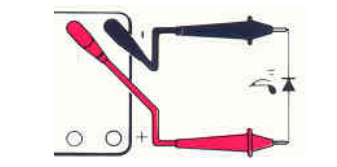
\includegraphics[width=3.5cm]{pictures/polaridad_multimetro1.png} & 
    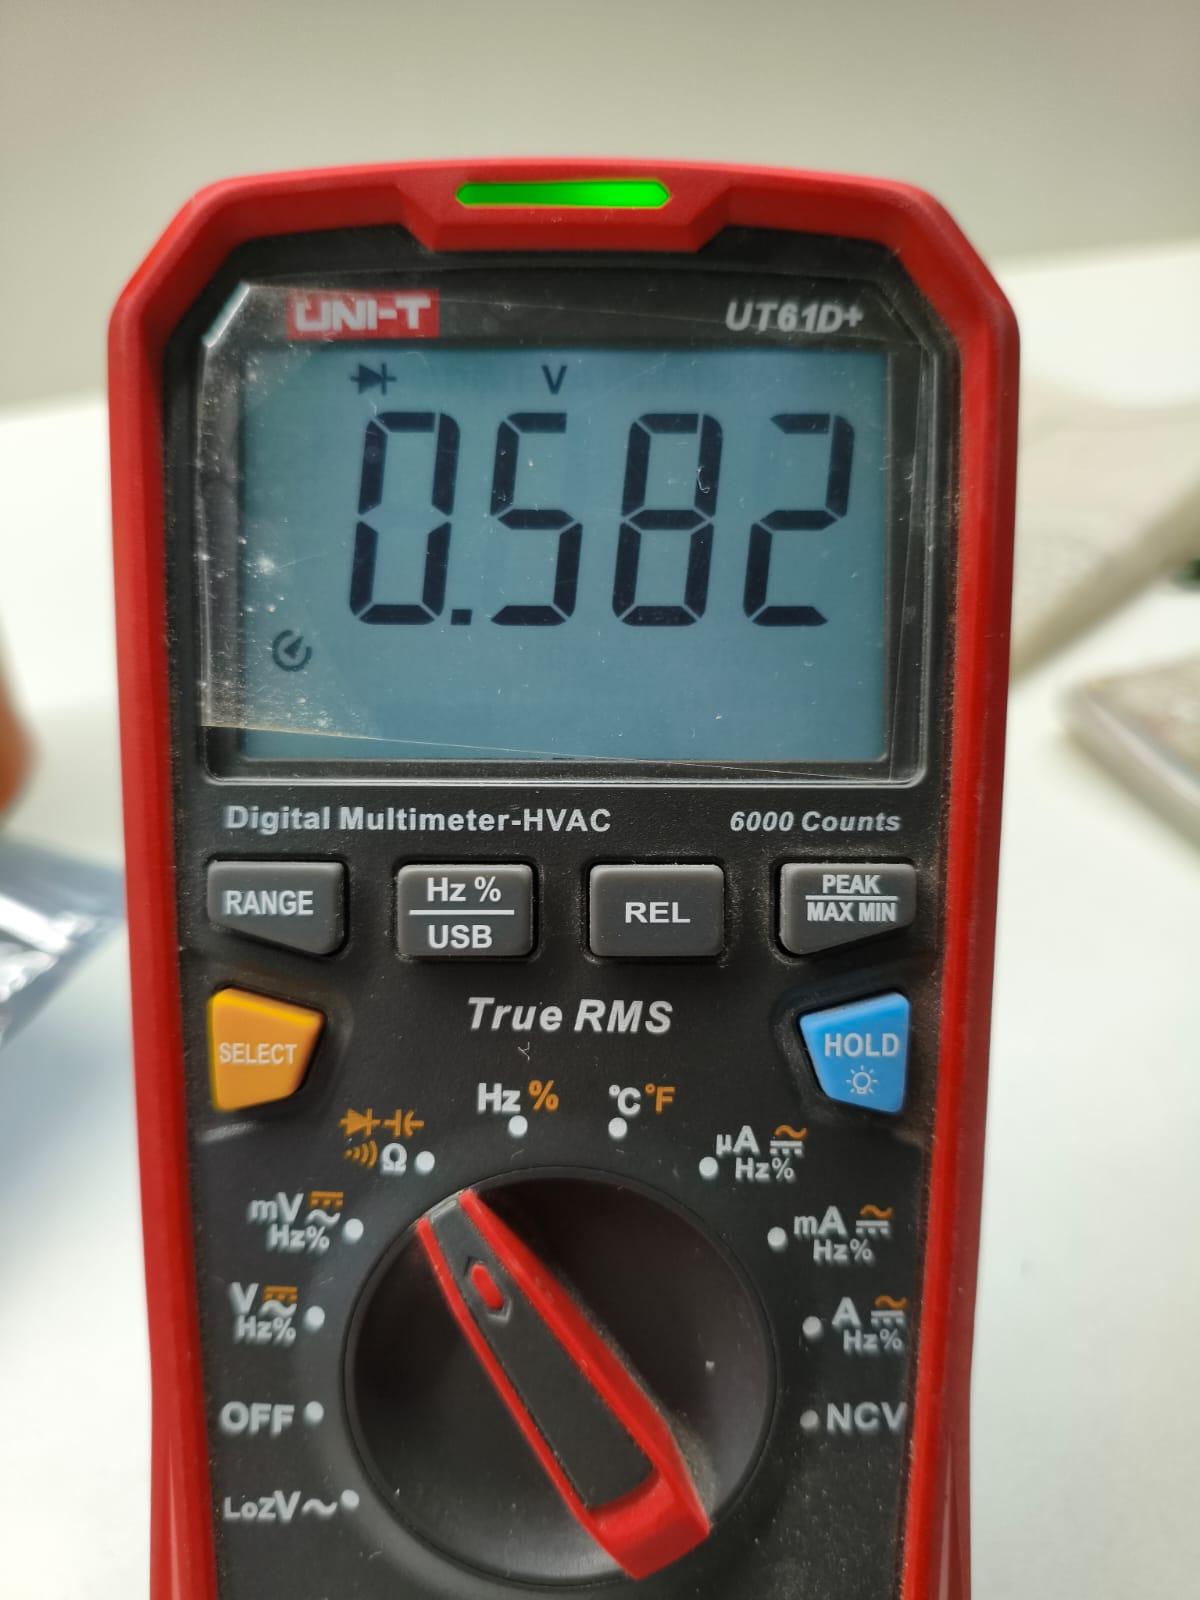
\includegraphics[width=\linewidth]{pictures/multimetro_silicio_directa.jpeg}
  & $0.592\V$ & $0.289\V$ & $0.293\V$  \\
  \hline
  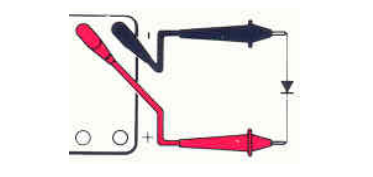
\includegraphics[width=3.5cm]{pictures/polaridad_multimetro2.png} & 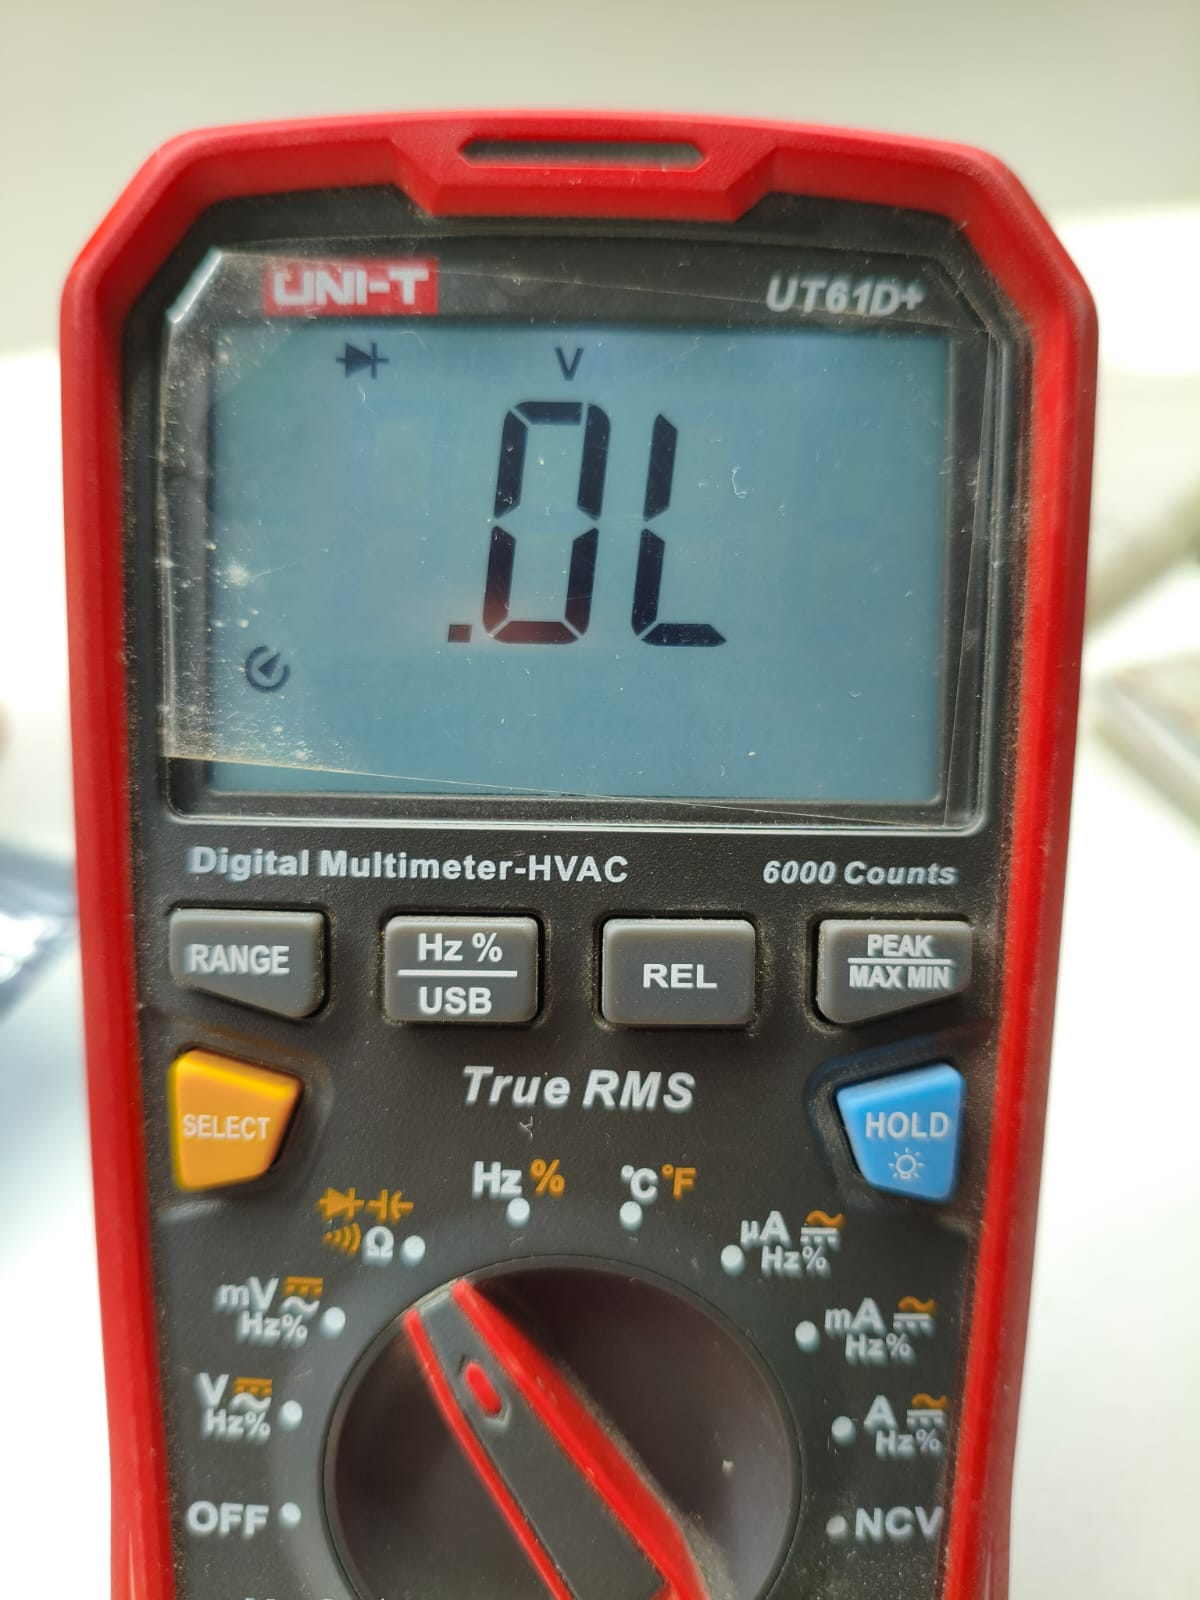
\includegraphics[width=\linewidth]{pictures/multimetro_silicio_inversa.jpeg}
  & Over limit & Over limit & Over limit  \\
  \hline
  \end{tabular}
  \caption{Resultados de las mediciones con el multimetro en modo diodo}
  \end{table}
  \end{center}

  \section{Conclusión}

  Se puede observar, que al medir en polarizacion directa, en el par de diodos de cada semiconductor, a pesar de ser el
  mismo modelo de diodo, no tienen la misma tension de barrera. Por otro lado, se comprueba que al medir en polarizacion
  inversa, la tension de barrera incrementa tanto que la herramienta simplemente no puede suministrar suficiente, por
  lo que marca "ol" lo cual significa "Over limit" o "por encima del limite" en español.




\chapter{Curva caracteristica del diodo}
    Los diodos son dispositivos semiconductores que permiten el paso de corriente en un único sentido. Su comportamiento se representa 
    gráficamente mediante la curva característica corriente–tensión (I-V), que muestra la relación entre la tensión aplicada y la 
    corriente que circula a través del diodo. En esta sección, se analiza este comportamiento tanto en diodos de silicio como de 
    germanio, enfocándonos en el punto de transición entre el estado de bloqueo (cuando el diodo no conduce) y el de conducción (cuando 
    permite el paso de corriente), conocido como tensión umbral. Para ello, se realizarán simulaciones y luego mediciones prácticas en el 
    laboratorio que permitirán comparar el desempeño real con los valores típicos indicados por los fabricantes.
    
  \section{Actividad de simulación}
    Se realizará esta actividad con el objetivo de observar en la plataforma de simulación LTspice la curva de los modelos de diodos que 
    utilizaremos para realizar ensayos en el laboratorio. A continuación, se presenta los circuitos implementados y las respectivas 
    gráficas obtenidas de la simulación. 

    \subsection{Polarización directa}
    \begin{figure}[H]
      \centering
      \begin{minipage}{0.45\textwidth}
        \centering
        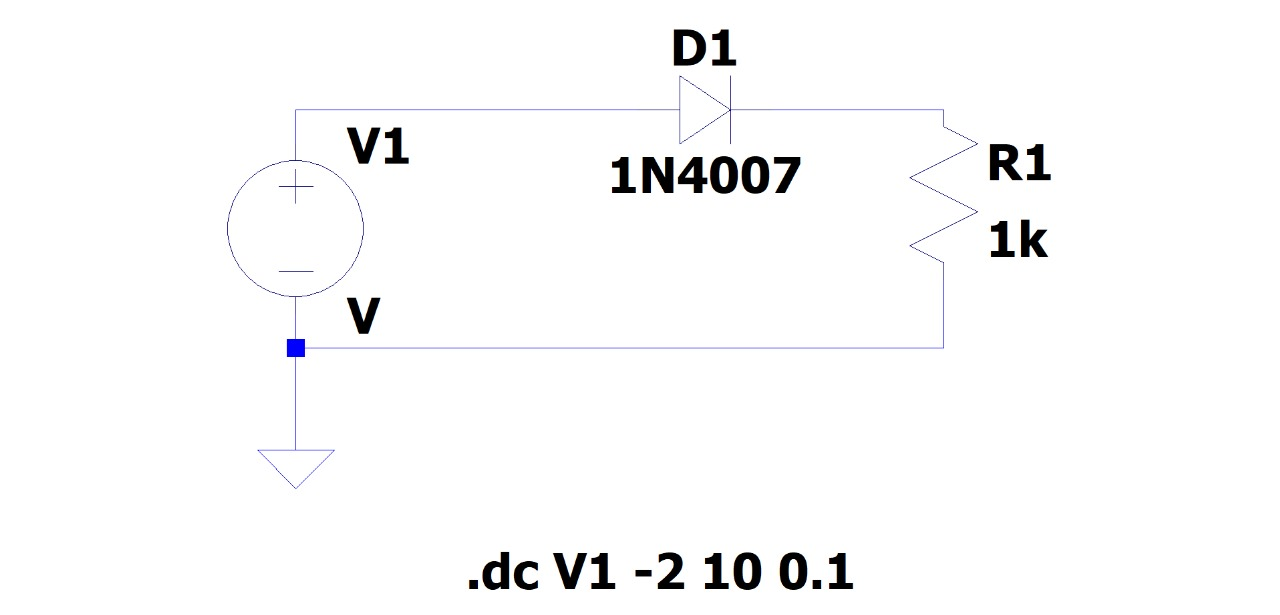
\includegraphics[width=\linewidth]{pictures/curva_diodo_silicio_circuito.jpeg}
        \captionof{figure}{Circuito básico del diodo de silicio 1N4007 en polarización directa.}
      \end{minipage}
      \hfill
      \begin{minipage}{0.45\textwidth}
        \centering
        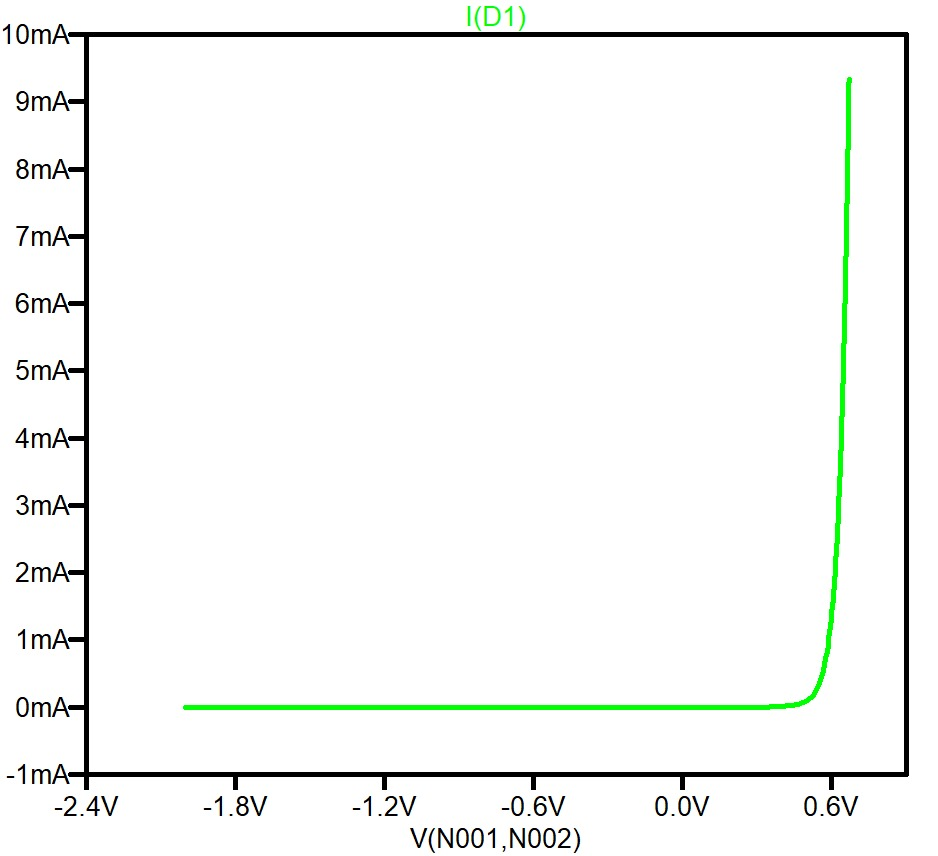
\includegraphics[width=\linewidth]{pictures/curva_diodo_silicio_grafico.jpeg}
        \captionof{figure}{Gráfica $I_D$ vs $V_D$ obtenida de la simulación.}
      \end{minipage}
      \vspace{0.5cm}
      \label{c}
    \end{figure}
    \begin{figure}[H]
        \centering
        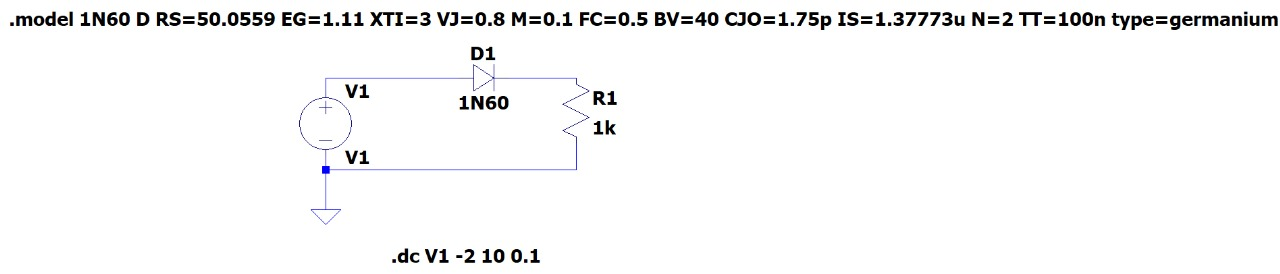
\includegraphics[width=\linewidth]{pictures/curva_diodo_germanio_circuito.jpeg}
        \caption{Circuito básico del diodo de germanio 1N60 en polarización directa.}
    \end{figure}
    \begin{figure}[H]
        \centering
        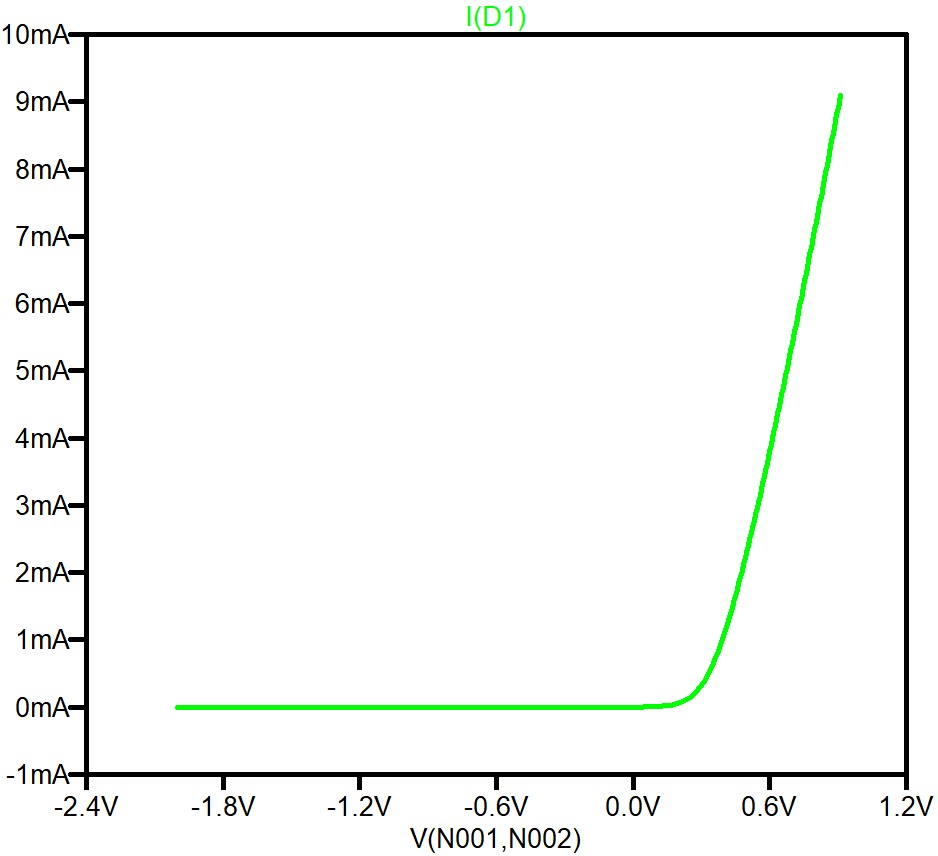
\includegraphics[width=0.5\linewidth]{pictures/curva_diodo_germanio_grafico.jpeg}
        \caption{Gráfica $I_D$ vs $V_D$ obtenida de la simulación.}

    \end{figure}

    Ambas simulaciones se han configurado de modo que se haga un barrido la fuente desde -2V a 10V, con un paso de 100mV 
    por cada punto a simular.

    A continuación, se muestra una gráfica con las dos curvas de los diodos, a modo de comparación:

    \begin{figure}[H]
        \centering
        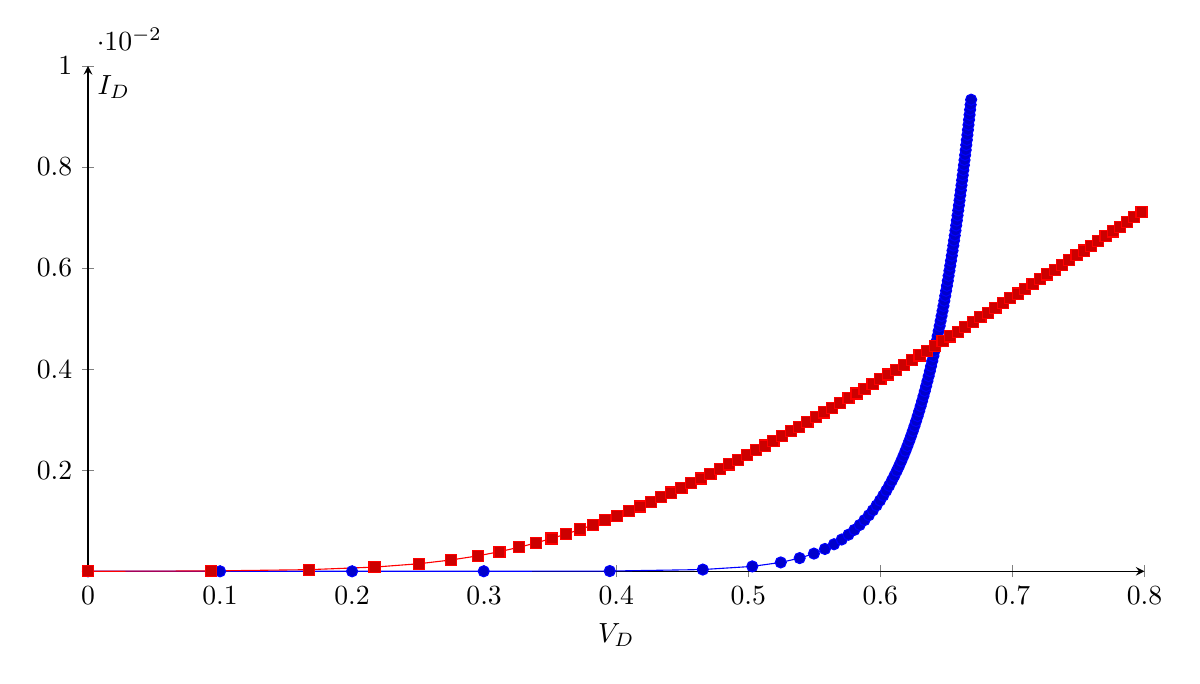
\begin{tikzpicture}
        \begin{axis}[
            xlabel={$V_D$},
            ylabel={$I_D$},
            axis lines = left,
            axis y line=middle,
            width=15cm,
            height=8cm,
            ymin=0, ymax=0.01,
            xmin=0, xmax=0.8,
        ]
        \addplot coordinates {
            (-9.999999e-01, -9.099665e-11)
            (-8.999999e-01, -9.089673e-11)
            (-7.999999e-01, -9.079681e-11)
            (-6.999999e-01, -9.069689e-11)
            (-5.999999e-01, -9.060253e-11)
            (-4.999999e-01, -9.049983e-11)
            (-3.999999e-01, -9.039852e-11)
            (-2.999999e-01, -9.027779e-11)
            (-1.999999e-01, -8.984063e-11)
            (-9.999991e-02, -8.441338e-11)
            (2.141297e-19, -2.141297e-22)
            (9.999867e-02, 1.334306e-09)
            (1.999776e-01, 2.243526e-08)
            (2.996469e-01, 3.531179e-07)
            (3.950736e-01, 4.926428e-06)
            (4.655261e-01, 3.447394e-05)
            (5.030010e-01, 9.699905e-05)
            (5.245518e-01, 1.754482e-04)
            (5.388615e-01, 2.611385e-04)
            (5.496788e-01, 3.503212e-04)
            (5.580088e-01, 4.419912e-04)
            (5.648770e-01, 5.351230e-04)
            (5.707332e-01, 6.292668e-04)
            (5.758181e-01, 7.241819e-04)
            (5.803047e-01, 8.196952e-04)
            (5.843167e-01, 9.156833e-04)
            (5.879430e-01, 1.012057e-03)
            (5.912504e-01, 1.108750e-03)
            (5.942897e-01, 1.205710e-03)
            (5.971005e-01, 1.302900e-03)
            (5.997144e-01, 1.400286e-03)
            (6.021570e-01, 1.497843e-03)
            (6.044491e-01, 1.595551e-03)
            (6.066080e-01, 1.693392e-03)
            (6.086482e-01, 1.791352e-03)
            (6.105821e-01, 1.889418e-03)
            (6.124201e-01, 1.987580e-03)
            (6.141711e-01, 2.085829e-03)
            (6.158430e-01, 2.184157e-03)
            (6.174426e-01, 2.282557e-03)
            (6.189759e-01, 2.381024e-03)
            (6.204481e-01, 2.479552e-03)
            (6.218638e-01, 2.578136e-03)
            (6.232273e-01, 2.676773e-03)
            (6.245422e-01, 2.775458e-03)
            (6.258119e-01, 2.874188e-03)
            (6.270394e-01, 2.972961e-03)
            (6.282273e-01, 3.071773e-03)
            (6.293781e-01, 3.170622e-03)
            (6.304942e-01, 3.269506e-03)
            (6.315774e-01, 3.368423e-03)
            (6.326298e-01, 3.467370e-03)
            (6.336529e-01, 3.566347e-03)
            (6.346484e-01, 3.665352e-03)
            (6.356177e-01, 3.764382e-03)
            (6.365622e-01, 3.863438e-03)
            (6.374831e-01, 3.962517e-03)
            (6.383815e-01, 4.061618e-03)
            (6.392586e-01, 4.160741e-03)
            (6.401153e-01, 4.259885e-03)
            (6.409525e-01, 4.359047e-03)
            (6.417712e-01, 4.458229e-03)
            (6.425720e-01, 4.557428e-03)
            (6.433558e-01, 4.656644e-03)
            (6.441234e-01, 4.755876e-03)
            (6.448752e-01, 4.855125e-03)
            (6.456121e-01, 4.954388e-03)
            (6.463345e-01, 5.053665e-03)
            (6.470430e-01, 5.152957e-03)
            (6.477382e-01, 5.252262e-03)
            (6.484205e-01, 5.351579e-03)
            (6.490904e-01, 5.450909e-03)
            (6.497484e-01, 5.550252e-03)
            (6.503948e-01, 5.649605e-03)
            (6.510301e-01, 5.748970e-03)
            (6.516547e-01, 5.848345e-03)
            (6.522689e-01, 5.947731e-03)
            (6.528730e-01, 6.047127e-03)
            (6.534674e-01, 6.146532e-03)
            (6.540523e-01, 6.245947e-03)
            (6.546282e-01, 6.345372e-03)
            (6.551952e-01, 6.444805e-03)
            (6.557536e-01, 6.544246e-03)
            (6.563038e-01, 6.643696e-03)
            (6.568458e-01, 6.743154e-03)
            (6.573800e-01, 6.842620e-03)
            (6.579066e-01, 6.942093e-03)
            (6.584258e-01, 7.041574e-03)
            (6.589378e-01, 7.141062e-03)
            (6.594428e-01, 7.240557e-03)
            (6.599411e-01, 7.340059e-03)
            (6.604326e-01, 7.439567e-03)
            (6.609178e-01, 7.539082e-03)
            (6.613967e-01, 7.638603e-03)
            (6.618694e-01, 7.738131e-03)
            (6.623362e-01, 7.837663e-03)
            (6.627972e-01, 7.937203e-03)
            (6.632525e-01, 8.036748e-03)
            (6.637022e-01, 8.136298e-03)
            (6.641466e-01, 8.235853e-03)
            (6.645857e-01, 8.335414e-03)
            (6.650196e-01, 8.434980e-03)
            (6.654485e-01, 8.534552e-03)
            (6.658726e-01, 8.634128e-03)
            (6.662918e-01, 8.733708e-03)
            (6.667064e-01, 8.833294e-03)
            (6.671163e-01, 8.932884e-03)
            (6.675218e-01, 9.032479e-03)
            (6.679229e-01, 9.132077e-03)
            (6.683197e-01, 9.231680e-03)
            (6.687123e-01, 9.331288e-03)
        };
        \addplot coordinates {
            (-1.998622e+00, -1.377732e-06)
            (-1.898622e+00, -1.377732e-06)
            (-1.798622e+00, -1.377732e-06)
            (-1.698622e+00, -1.377732e-06)
            (-1.598622e+00, -1.377732e-06)
            (-1.498622e+00, -1.377731e-06)
            (-1.398622e+00, -1.377731e-06)
            (-1.298622e+00, -1.377731e-06)
            (-1.198622e+00, -1.377731e-06)
            (-1.098622e+00, -1.377731e-06)
            (-9.986223e-01, -1.377731e-06)
            (-8.986223e-01, -1.377731e-06)
            (-7.986223e-01, -1.377731e-06)
            (-6.986223e-01, -1.377729e-06)
            (-5.986223e-01, -1.377718e-06)
            (-4.986224e-01, -1.377641e-06)
            (-3.986229e-01, -1.377109e-06)
            (-2.986266e-01, -1.373438e-06)
            (-1.986519e-01, -1.348084e-06)
            (-9.882643e-02, -1.173573e-06)
            (2.152422e-14, -2.152422e-17)
            (9.310054e-02, 6.899460e-06)
            (1.674261e-01, 3.257387e-05)
            (2.170099e-01, 8.299015e-05)
            (2.504628e-01, 1.495372e-04)
            (2.751413e-01, 2.248587e-04)
            (2.950752e-01, 3.049248e-04)
            (3.115954e-01, 3.884046e-04)
            (3.260566e-01, 4.739434e-04)
            (3.390792e-01, 5.609208e-04)
            (3.510056e-01, 6.489944e-04)
            (3.620810e-01, 7.379189e-04)
            (3.724809e-01, 8.275192e-04)
            (3.823322e-01, 9.176678e-04)
            (3.917301e-01, 1.008270e-03)
            (4.007470e-01, 1.099253e-03)
            (4.094398e-01, 1.190560e-03)
            (4.178534e-01, 1.282147e-03)
            (4.260244e-01, 1.373976e-03)
            (4.339825e-01, 1.466017e-03)
            (4.417523e-01, 1.558248e-03)
            (4.493546e-01, 1.650645e-03)
            (4.568068e-01, 1.743193e-03)
            (4.641238e-01, 1.835876e-03)
            (4.713184e-01, 1.928682e-03)
            (4.784017e-01, 2.021598e-03)
            (4.853833e-01, 2.114617e-03)
            (4.922718e-01, 2.207728e-03)
            (4.990744e-01, 2.300926e-03)
            (5.057979e-01, 2.394202e-03)
            (5.124481e-01, 2.487552e-03)
            (5.190303e-01, 2.580970e-03)
            (5.255491e-01, 2.674451e-03)
            (5.320088e-01, 2.767991e-03)
            (5.384132e-01, 2.861587e-03)
            (5.447658e-01, 2.955234e-03)
            (5.510697e-01, 3.048930e-03)
            (5.573279e-01, 3.142672e-03)
            (5.635428e-01, 3.236457e-03)
            (5.697171e-01, 3.330283e-03)
            (5.758528e-01, 3.424147e-03)
            (5.819520e-01, 3.518048e-03)
            (5.880166e-01, 3.611983e-03)
            (5.940484e-01, 3.705952e-03)
            (6.000489e-01, 3.799951e-03)
            (6.060196e-01, 3.893980e-03)
            (6.119620e-01, 3.988038e-03)
            (6.178773e-01, 4.082123e-03)
            (6.237668e-01, 4.176233e-03)
            (6.296315e-01, 4.270369e-03)
            (6.354725e-01, 4.364527e-03)
            (6.412910e-01, 4.458709e-03)
            (6.470876e-01, 4.552912e-03)
            (6.528634e-01, 4.647137e-03)
            (6.586192e-01, 4.741381e-03)
            (6.643557e-01, 4.835644e-03)
            (6.700737e-01, 4.929926e-03)
            (6.757738e-01, 5.024226e-03)
            (6.814567e-01, 5.118543e-03)
            (6.871232e-01, 5.212877e-03)
            (6.927736e-01, 5.307226e-03)
            (6.984085e-01, 5.401591e-03)
            (7.040287e-01, 5.495972e-03)
            (7.096344e-01, 5.590366e-03)
            (7.152261e-01, 5.684774e-03)
            (7.208045e-01, 5.779196e-03)
            (7.263697e-01, 5.873630e-03)
            (7.319224e-01, 5.968078e-03)
            (7.374628e-01, 6.062537e-03)
            (7.429913e-01, 6.157008e-03)
            (7.485084e-01, 6.251492e-03)
            (7.540143e-01, 6.345986e-03)
            (7.595093e-01, 6.440490e-03)
            (7.649938e-01, 6.535006e-03)
            (7.704682e-01, 6.629532e-03)
            (7.759326e-01, 6.724067e-03)
            (7.813872e-01, 6.818613e-03)
            (7.868325e-01, 6.913167e-03)
            (7.922687e-01, 7.007731e-03)
            (7.976959e-01, 7.102304e-03)
        };
        \end{axis}
        \end{tikzpicture}
        \caption{\footnotesize
        Gráfica con las curvas $I_D$ vs $V_D$ (simulación) de los diodos de Silicio y Germanio.}
        \end{figure}

    \subsection{Polarización inversa}
    
    \begin{figure}[H]
      \centering
      \begin{minipage}{0.45\textwidth}
        \centering
        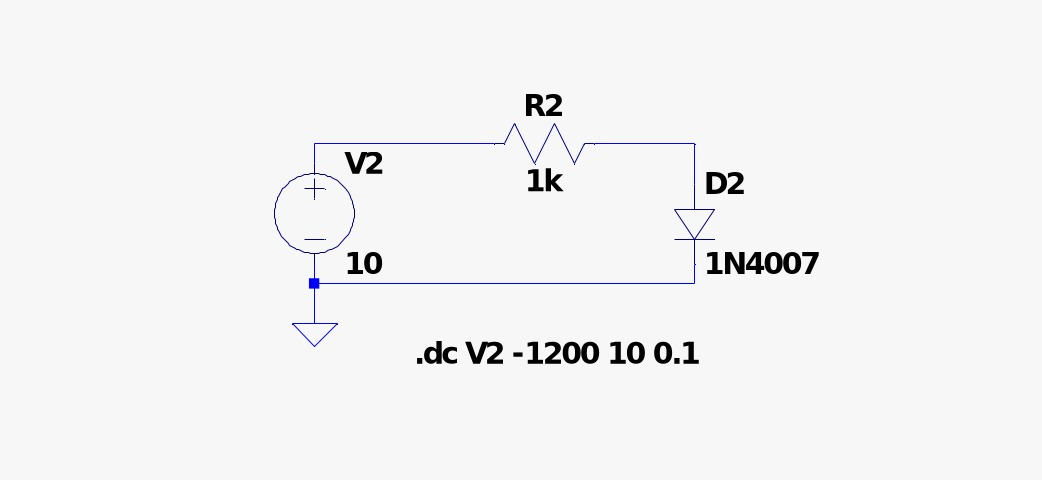
\includegraphics[width=\linewidth]{pictures/circuito_diodo_silicio_inversa.jpeg}
        \captionof{figure}{Circuito básico del diodo de silicio 1N4007 en polarización inversa.}
      \end{minipage}
      \hfill
      \begin{minipage}{0.45\textwidth}
        \centering
        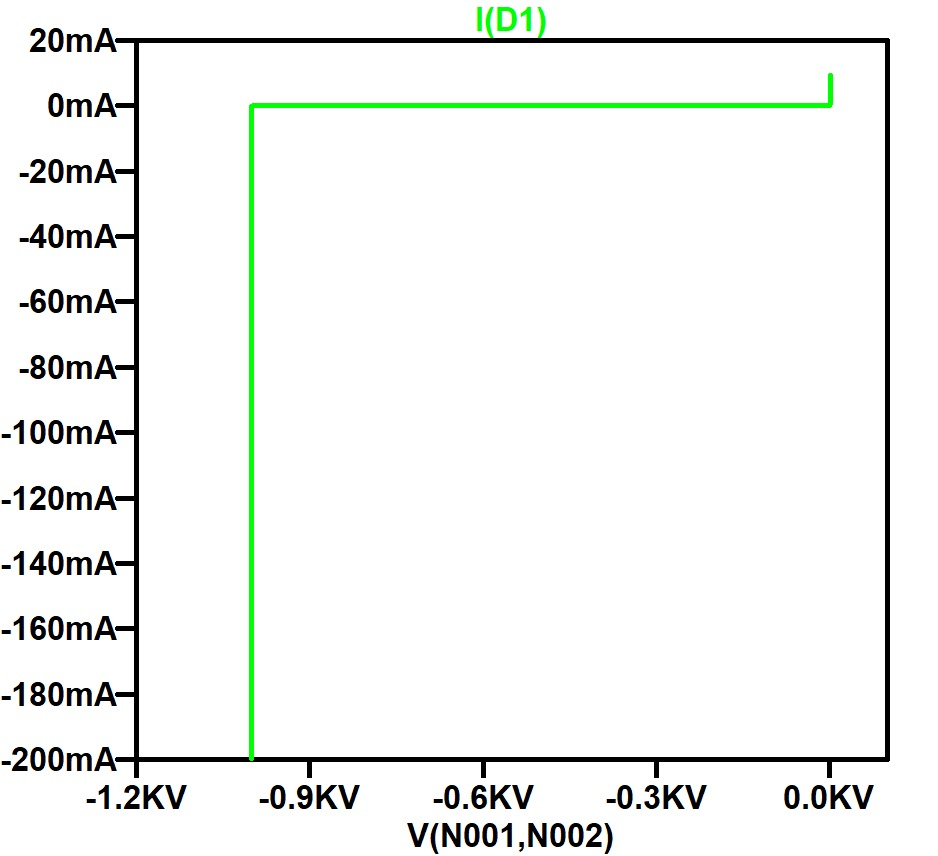
\includegraphics[width=\linewidth]{pictures/curva_diodo_silicio_inversa.jpeg}
        \captionof{figure}{Gráfica $I_D$ vs $V_D$ obtenida de la simulación.}
      \end{minipage}
    \end{figure}

    \begin{figure}[H]
      \centering
      \begin{minipage}{1\textwidth}
        \centering
        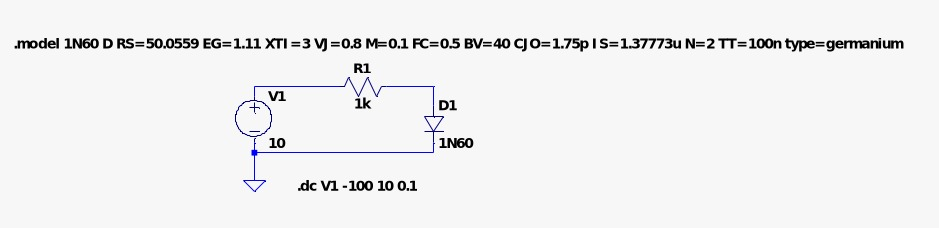
\includegraphics[width=\linewidth]{pictures/circuito_diodo_germanio_inversa.jpeg}
        \captionof{figure}{Circuito básico del diodo de germanio 1N60 en polarización inversa.}
      \end{minipage}
      \hfill
      \begin{minipage}{0.45\textwidth}
        \centering
        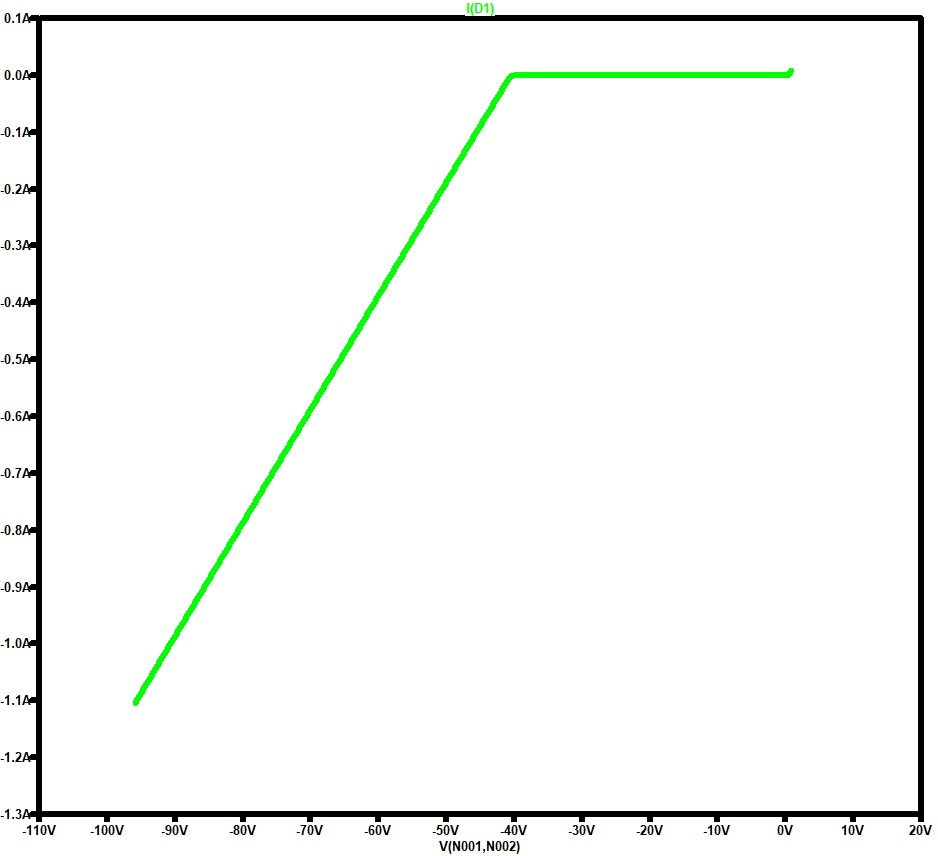
\includegraphics[width=\linewidth]{pictures/curva_diodo_germanio_inversa.jpeg}
        \captionof{figure}{Gráfica $I_D$ vs $V_D$ obtenida de la simulación.}
      \end{minipage}
    \end{figure}

    \subsection{Conclusión}
    Podemos concluir que la simulación es una herramienta muy útil, que sirve para observar el comportamiento de un dispositivo 
    electrónico y sacar ciertas conclusiones del mismo antes de implementarlo en el laboratorio o en un proyecto. Sin embargo, 
    es importante seleccionar modelos fieles en los circuitos implementados para simular. Por ejemplo, pudimos observar que el 
    modelo del diodo de germanio utilizado para la simulación presenta mucha variación de tensión a medida que aumenta la 
    corriente, lo cual suponemos que no es del todo correcto. Por otro lado, tuvimos resultados satisfactorios en la simulación 
    de los diodos polarizados en inversa. 

  \section{Actividad de laboratortio}
    En las clases teóricas se ha visto que el diodo no tiene un comportamiento lineal. Pudimos observar su 
    comportamiento no lineal en la simulación del inciso anterior. Ahora, lo observaremos en el laboratorio de la
    facultad, con el objetivo de comprobar la teoría y la simulación con la realidad. Para lograr esto, implementaremos
    el siguiente circuito:

    \begin{figure}[H]
        \centering
        \begin{tikzpicture}
    	% Paths, nodes and wires:
    	\draw (8.25, 4.5) to[empty diode, l={$D$}, label distance=0.02cm] (8.25, 2.75);
    	\draw (5.25, 4.75) to[american resistor, l={$R_D$}, label distance=0.02cm] (7.25, 4.75);
    	\draw (2.75, 2.75) to[voltmeter, l={$V_{in}$}, label distance=0.02cm] (2.75, 4.5);
    	\draw (9.75, 2.75) to[voltmeter, l_={$V_d$}, label distance=0.02cm] (9.75, 4.5);
    	\draw (5.25, 2.5) to[ammeter, l={$I_D$}, label distance=0.02cm] (7.25, 2.5);
    	\draw (4.25, 4.5) -| (4.25, 4.75) -- (5.25, 4.75);
    	\draw (4.25, 2.75) -| (4.25, 2.5) -- (5.25, 2.5);
    	\draw (7.25, 4.75) -- (8.25, 4.75) -| (8.25, 4.5);
    	\draw (7.25, 2.5) -- (8.25, 2.5) -| (8.25, 2.75);
    	\draw (8.25, 4.75) -- (9.75, 4.75) -| (9.75, 4.5);
    	\draw (8.25, 2.5) -| (9.75, 2.75);
    	\draw (2.75, 4.5) -| (2.75, 4.75) -- (4.25, 4.75);
    	\draw (2.75, 2.75) -| (2.75, 2.5) -- (4.25, 2.5);
    	\draw (4.25, 4.5) to[battery1, l={$V$}, label distance=0.02cm] (4.25, 2.75);
        \end{tikzpicture}
        \caption{\footnotesize
        Circuito básico del diodo en polarización directa con los instrumentos de medición.}
    \end{figure}

    En este circuito, $V$ es una fuente de tensión variable, con la cual alimentaremos el circuito para analizar el 
    comportamiento del diodo en varios puntos y así poder trazar una curva de características del mismo. Se han tomado
    10 puntos, partiendo de 0V hasta 5V.
    
    A continuación, se presenta una tabla, tanto para el diodo de $Si$ como para el de $Ge$, con los valores obtenidos 
    de $V_D$ e $I_D$ para los distintos valores de alimentación. También, se presenta una gráfica de las curvas de 
    características obtenidas para ambos diodos y, fotografías de los instrumentos de medición utilizados y disposición 
    de los circuitos:
  
    \subsubsection{Diodo de silicio}
    
      \begin{table}[H]
      \centering 
      \renewcommand{\arraystretch}{1.5}
      \setlength{\tabcolsep}{8pt}
      \resizebox{\textwidth}{!}{
      \begin{tabular}{|c|*{13}{c|}}
      \hline
      \textbf{$V_1$ [V]} & 0 & 0.098 & 0.304 & 0.399 & \cellcolor{yellow}0.448 & \cellcolor{yellow}0.491 & \cellcolor{yellow}0.548 & \cellcolor{yellow}0.599 & \cellcolor{yellow}0.653 & \cellcolor{yellow}0.693 & 1.047 & 3.028 & 5.037 \\
      \hline
      $V_D[V]$ & 0 & 0.097 & 0.29 & 0.37 & 0.4 & 0.42 & 0.44 & 0.46 & 0.48 & 0.48 & 0.53 & 0.61 & 0.64 \\
      \hline
      $I_D[mA]$ & 0 & 0 & 0 & 0 & 0 & 0.053 & 0.087 & 0.124 & 0.165 & 0.196 & 0.511 & 2.4 & 4.4 \\
      \hline
      \end{tabular}
      }
      \caption{Tabla de valores $V_D$ e $I_D$ para diodo de silicio 1N4007.}
      \label{a}
      \end{table}
    
    \subsubsection{Diodo de germanio}
      \begin{table}[H]
      \centering
      \renewcommand{\arraystretch}{1.5}
      \setlength{\tabcolsep}{8pt}
      \resizebox{\textwidth}{!}{
      \begin{tabular}{|c|*{13}{c|}}
      \hline
      \textbf{$V_1$ [V]} & 0.051 & 0.103 & 0.154 & 0.201 & \cellcolor{yellow}0.245 & \cellcolor{yellow}0.301 & \cellcolor{yellow}0.344 & \cellcolor{yellow}0.674 & \cellcolor{yellow}0.694 & \cellcolor{yellow}0.907 & 1.5 & 3 & 5 \\
      \hline
      $V_D[V]$ & 0.04 & 0.08 & 0.13 & 0.16 & 0.18 & 0.19 & 0.22 & 0.26 & 0.24 & 0.26 & 0.28 & 0.32 & 0.35 \\
      \hline
      $I_D[mA]$ & 0.0006 & 0.0027 & 0.012 & 0.029 & 0.055 & 0.1 & 0.19 & 0.68 & 0.4 & 0.6 & 1.2 & 2.7 & 4.7 \\
      \hline
      \end{tabular}
      }
      \caption{Tabla de valores $V_D$ e $I_D$ para diodo de germanio 1N60.}
      \label{b}
      \end{table}

    \subsubsection{Curvas $I_D$ vs $V_D$}
    \begin{figure}[H]
        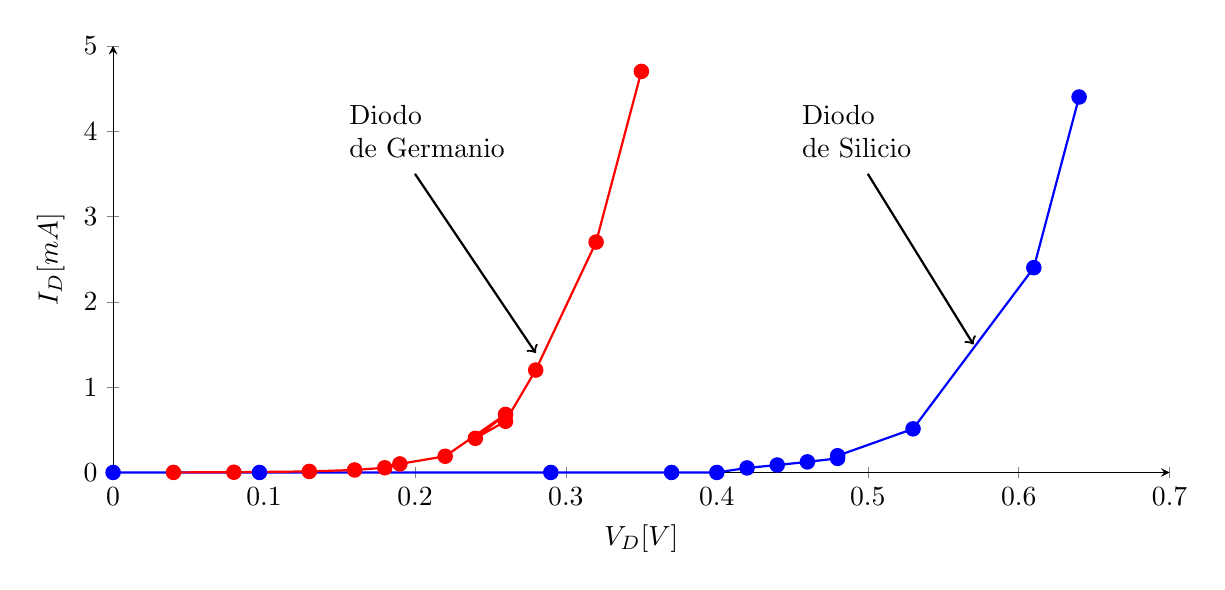
\begin{tikzpicture}
          \begin{axis}[
            axis lines = left,
            ylabel = {$I_{D}[mA]$},
            xlabel = {$V_{D}[V]$},
            width=15cm,
            height=7cm,
            ymin=0, ymax=5,
            xmin=0, xmax=0.7,
            ytick={0,1,2,3,4,5},
            xtick={0,0.1,0.2,0.3,0.4,0.5,0.6,0.7},
            clip=false, % necesario para dibujar fuera del área del gráfico
          ]
            % DIODO SILICIO
            \addplot[
              color=blue,
              mark=*,
              only marks,
              mark options={scale=1.3}
            ]
            coordinates {
                (0, 0)
                (0.097, 0)
                (0.29, 0)
                (0.37, 0)
                (0.4, 0)
                (0.42, 0.053)
                (0.44, 0.087)
                (0.46, 0.124)
                (0.48, 0.165)
                (0.48, 0.196)
                (0.53, 0.511)
                (0.61, 2.4)
                (0.64, 4.4)
            };
            \addplot[
              color=blue,
              thick
            ]
            coordinates {
                (0, 0)
                (0.097, 0)
                (0.29, 0)
                (0.37, 0)
                (0.4, 0)
                (0.42, 0.053)
                (0.44, 0.087)
                (0.46, 0.124)
                (0.48, 0.165)
                (0.48, 0.196)
                (0.53, 0.511)
                (0.61, 2.4)
                (0.64, 4.4)
            };
            \node[align=left, anchor=west] at (axis cs:0.45,4) {Diodo\\de Silicio};
            \draw[->, thick] (axis cs:0.5,3.5) -- (axis cs:0.57,1.5);
            % FIN DIODO SILICIO
            % DIODO GERMANIO
            \addplot[
              color=red,
              mark=*,
              only marks,
              mark options={scale=1.3}
            ]
            coordinates {
                (0.04, 0.0006)
                (0.08, 0.0027)
                (0.13, 0.012)
                (0.16, 0.029)
                (0.18, 0.055)
                (0.19, 0.1)
                (0.22, 0.19)
                (0.26, 0.68)
                (0.24, 0.4)
                (0.26, 0.6)
                (0.28, 1.2)
                (0.32, 2.7)
                (0.35, 4.7)
            };
            \addplot[
              color=red,
              thick
            ]
            coordinates {
                (0.04, 0.0006)
                (0.08, 0.0027)
                (0.13, 0.012)
                (0.16, 0.029)
                (0.18, 0.055)
                (0.19, 0.1)
                (0.22, 0.19)
                (0.26, 0.68)
                (0.24, 0.4)
                (0.26, 0.6)
                (0.28, 1.2)
                (0.32, 2.7)
                (0.35, 4.7)
            };
            \node[align=left, anchor=west] at (axis cs:0.15,4) {Diodo\\de Germanio};
            \draw[->, thick] (axis cs:0.2,3.5) -- (axis cs:0.28,1.4);
            % FIN DIODO GERMANIO
          \end{axis}
        \end{tikzpicture}
        \caption{\footnotesize
        Gráfica con las curvas $I_D$ vs $V_D$ (medidos en el laboratorio) de los diodos de Silicio y Germanio.}
        \end{figure}
      
    \subsubsection{Fotografías}
      \begin{figure}[H]
        \centering
        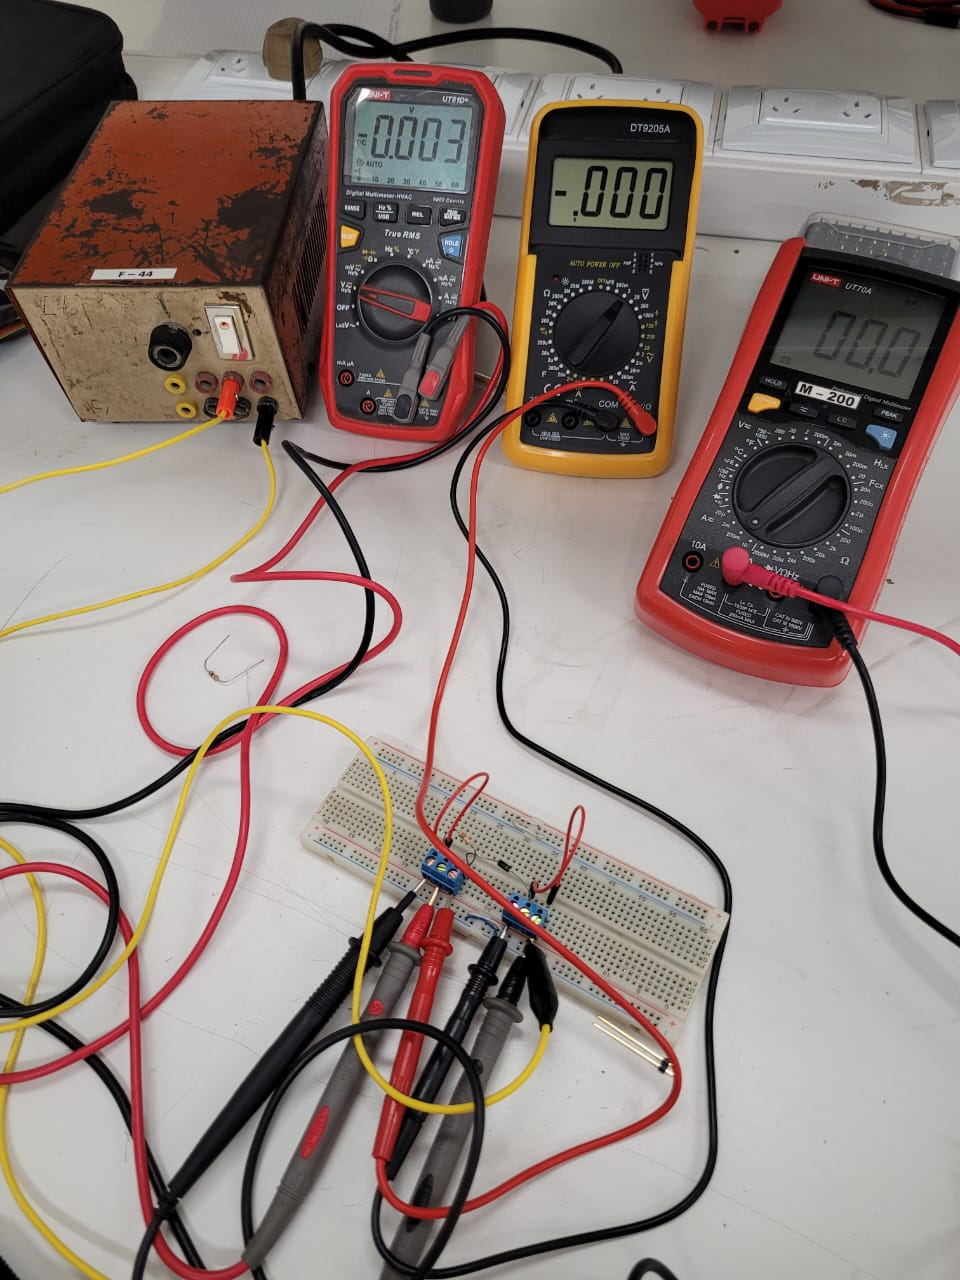
\includegraphics[width=.35\textwidth]{pictures/disposicion-elementos.jpeg}
        \caption{Fotografía general de los elementos utilizados para los ensayos.}
      \end{figure}
      \begin{figure}[H]
        \centering
        \begin{minipage}{0.40\textwidth}
            \centering
            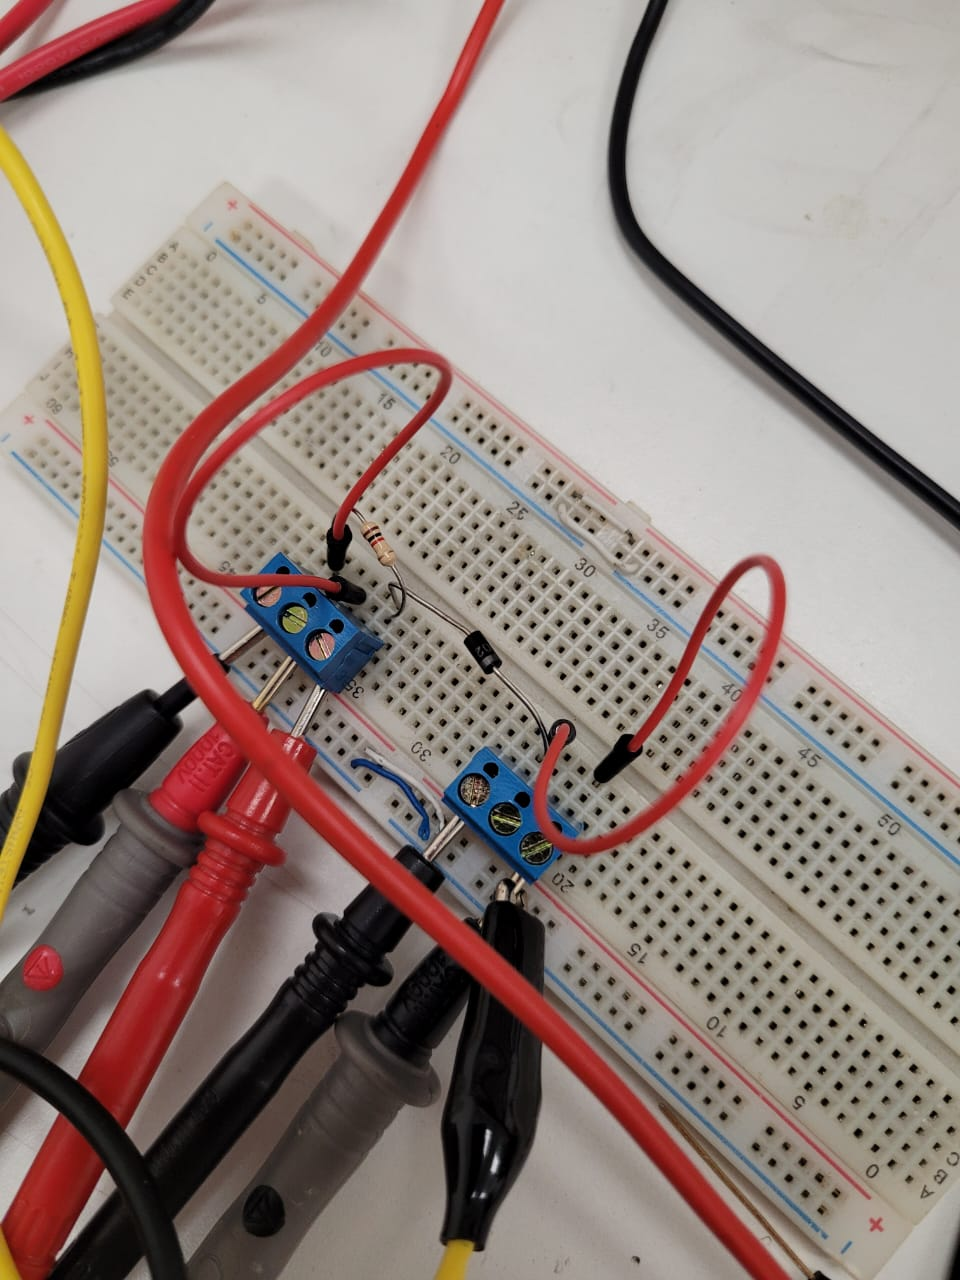
\includegraphics[width=\textwidth]{pictures/disposicion-circuito-silicio.jpeg}
            \caption{Disposición de los elementos del circuito. Diodo de Silicio.}
            \label{fig:silicio}
        \end{minipage}
        \hspace{0.05\textwidth} % Espacio entre imágenes
        \begin{minipage}{0.5\textwidth}
            \centering
            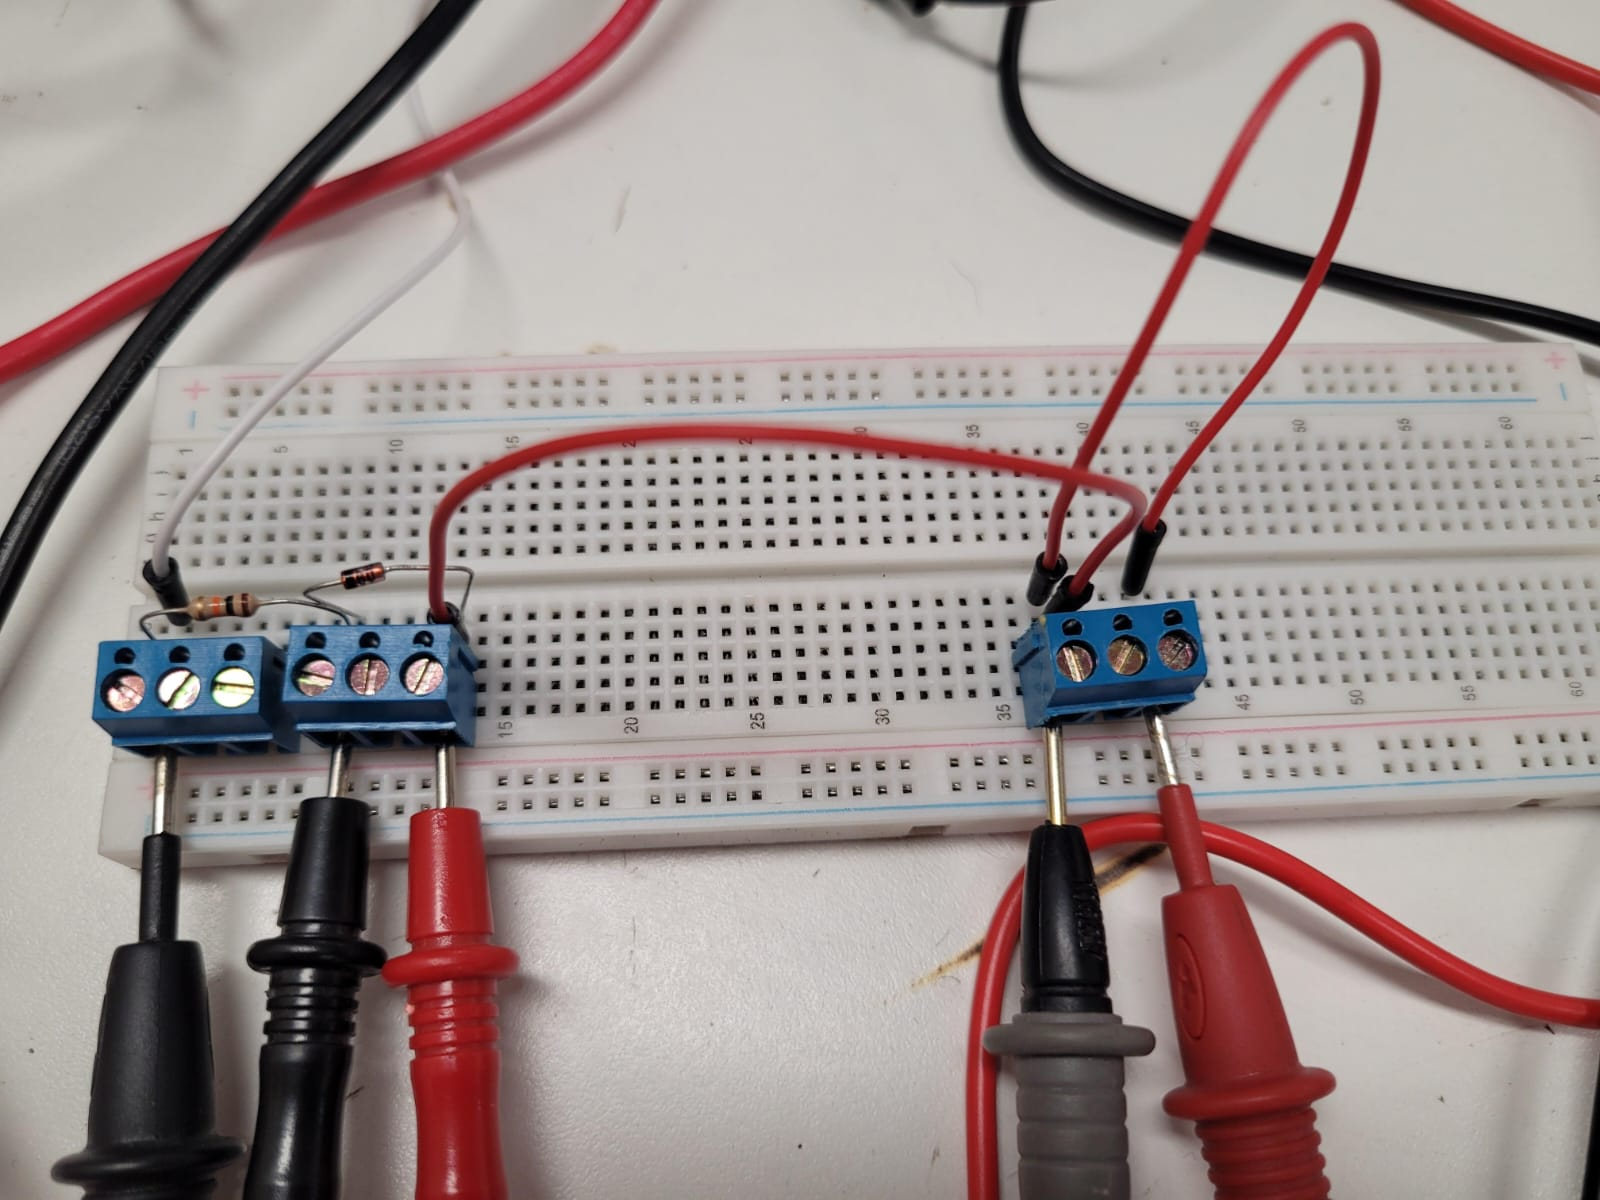
\includegraphics[width=\textwidth]{pictures/disposicion-circuito-germanio.jpeg}
            \caption{Disposición de los elementos del circuito. Diodo de Germanio.}
            \label{fig:germanio}
        \end{minipage}
    \end{figure}
    \begin{figure}[H]
        \centering
        \begin{minipage}{0.3\textwidth}
            \centering
            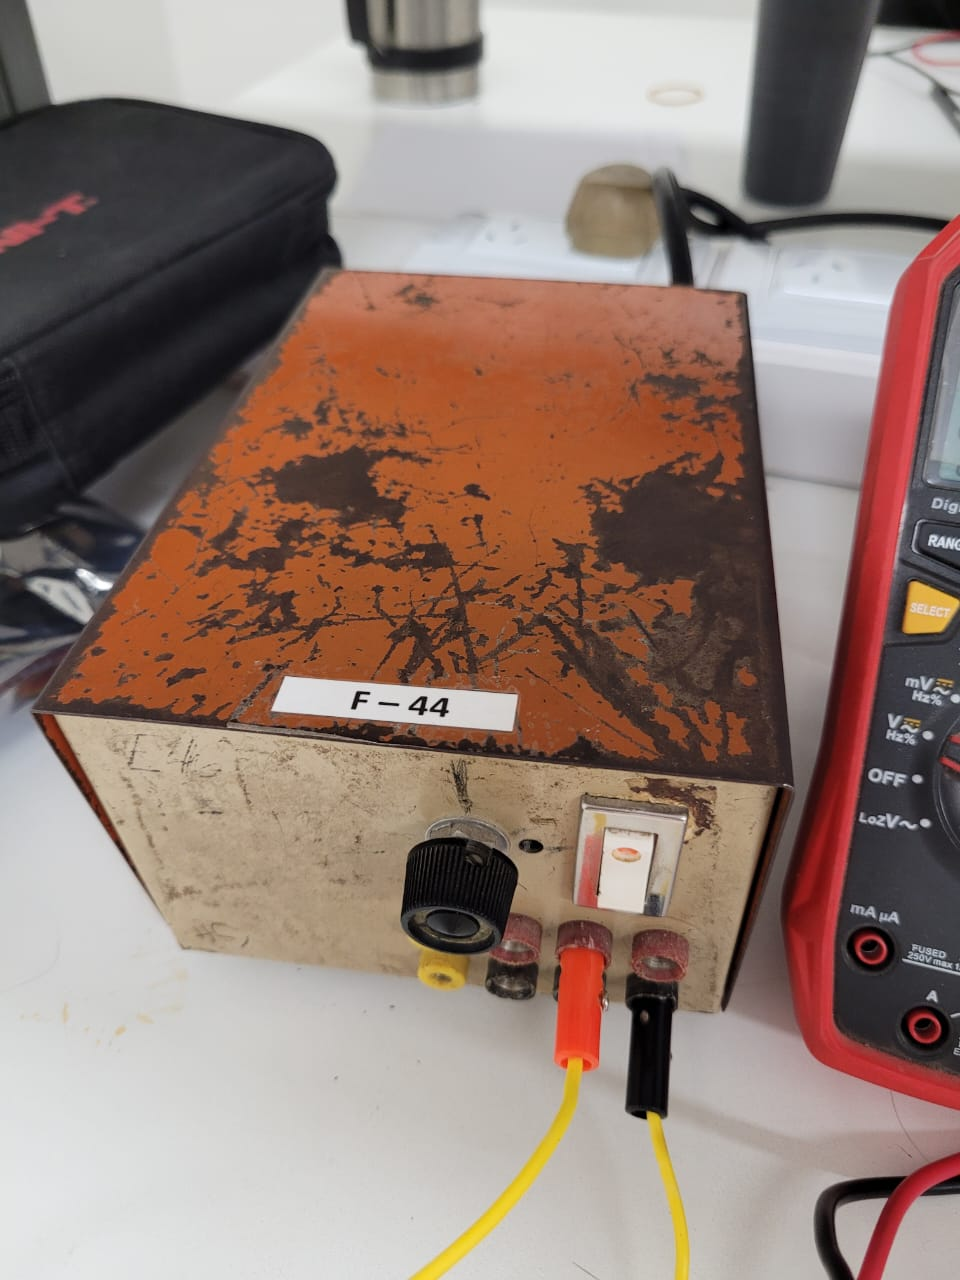
\includegraphics[width=\textwidth]{pictures/fuentealim.jpeg}
            \caption{Instrumentos: fuente de alimentación proporcionado por el laboratorio. Número de identificación: F-44}
        \end{minipage}
        \hspace{0.05\textwidth} % Espacio entre imágenes
        \begin{minipage}{0.3\textwidth}
            \centering
            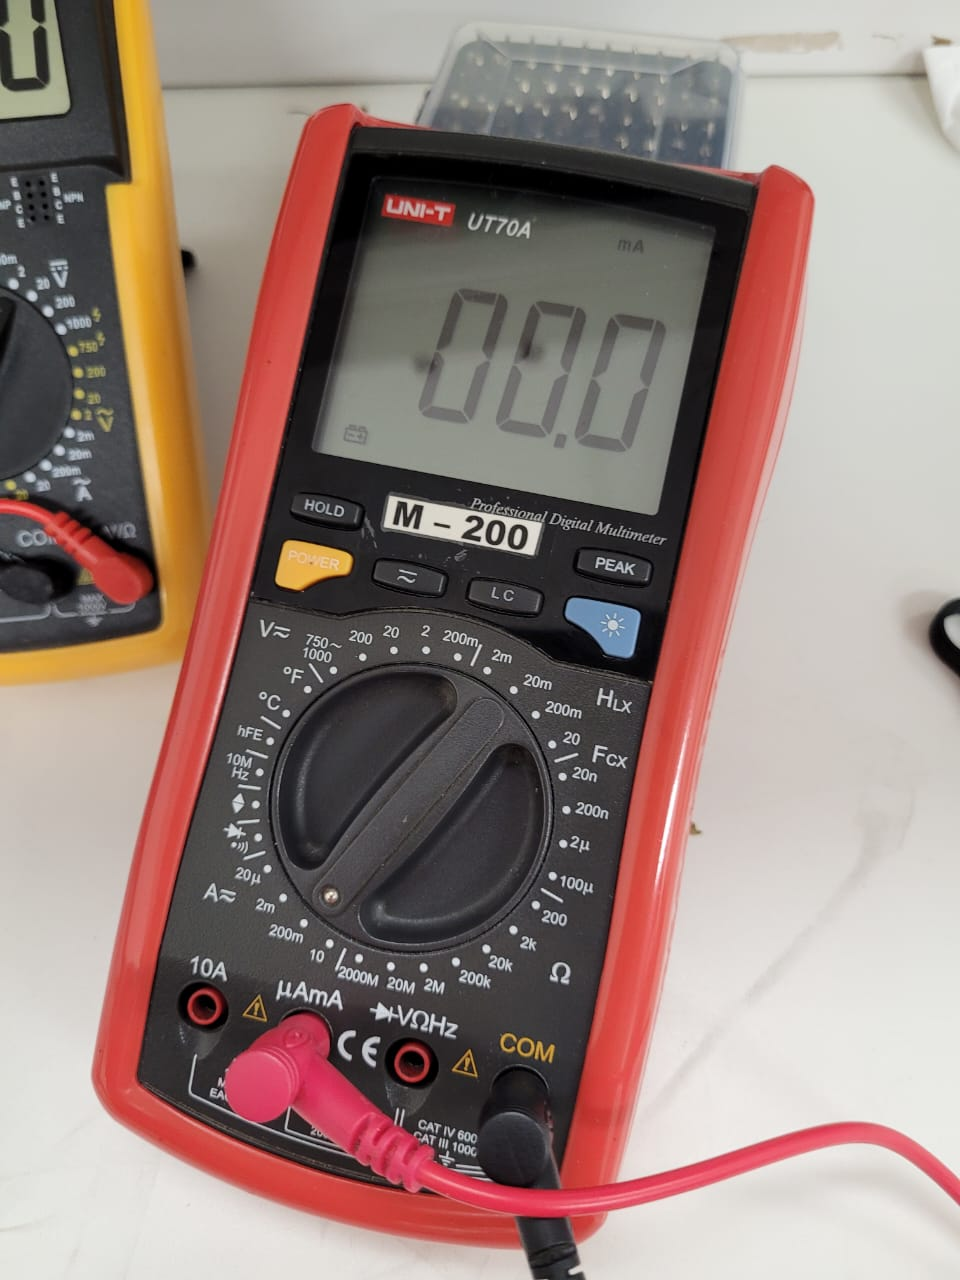
\includegraphics[width=\textwidth]{pictures/multimetro-facu.jpeg}
            \caption{Instrumentos: multimétro digital Nº1, proporcionado por el laboratorio marca UNI-T modelo UT70A. Número de identificación: M-200}
        \end{minipage}
    \end{figure}
    \begin{figure}[H]
        \centering
        \begin{minipage}{0.3\textwidth}
            \centering
            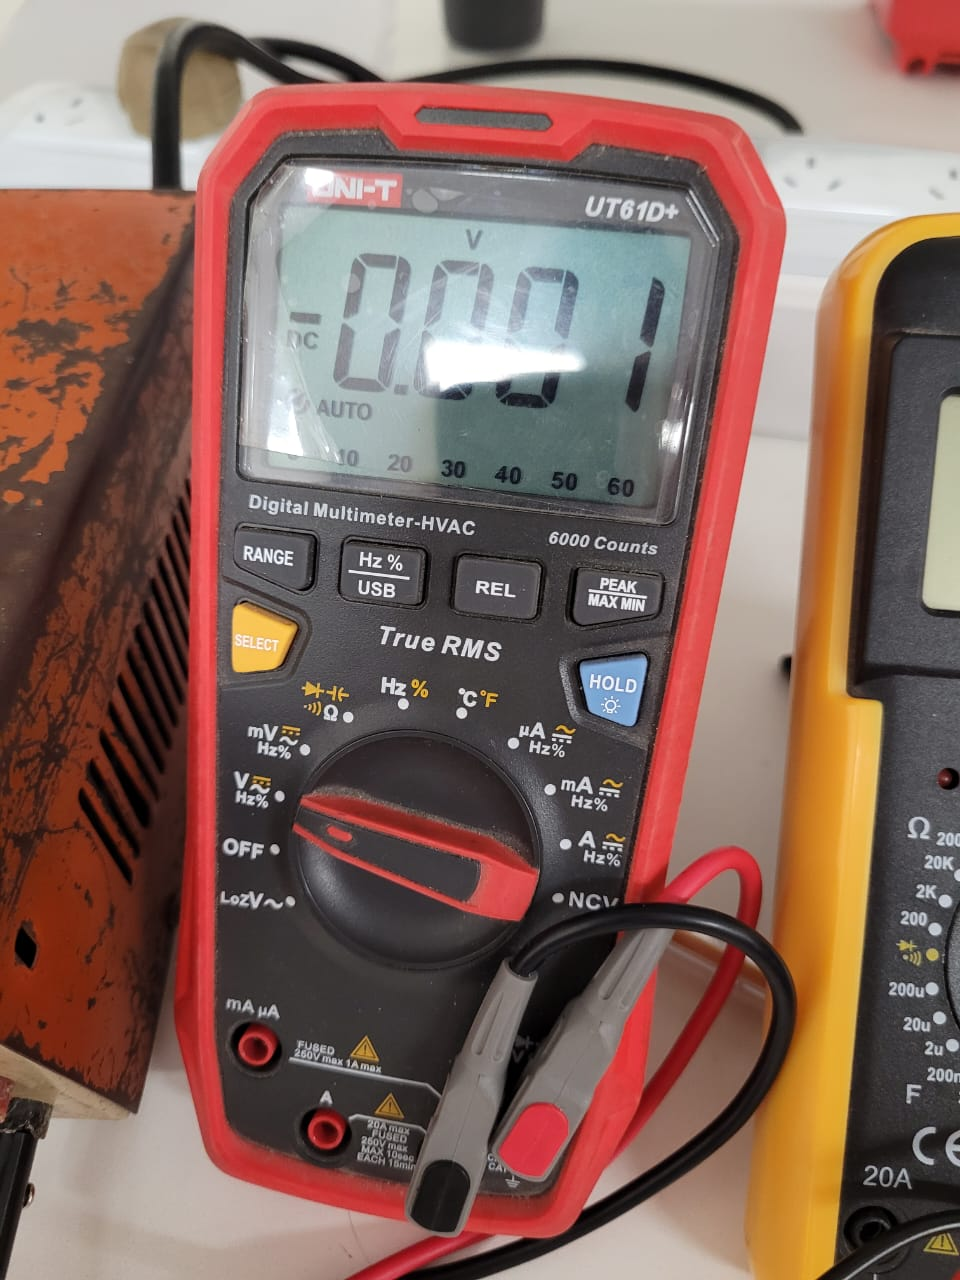
\includegraphics[width=\textwidth]{pictures/multimetro-gaston.jpeg}
            \caption{Instrumentos: multimétro digital Nº2, marca UNI-T modelo UT61D+.}
        \end{minipage}
        \hspace{0.05\textwidth} % Espacio entre imágenes
        \begin{minipage}{0.3\textwidth}
            \centering
            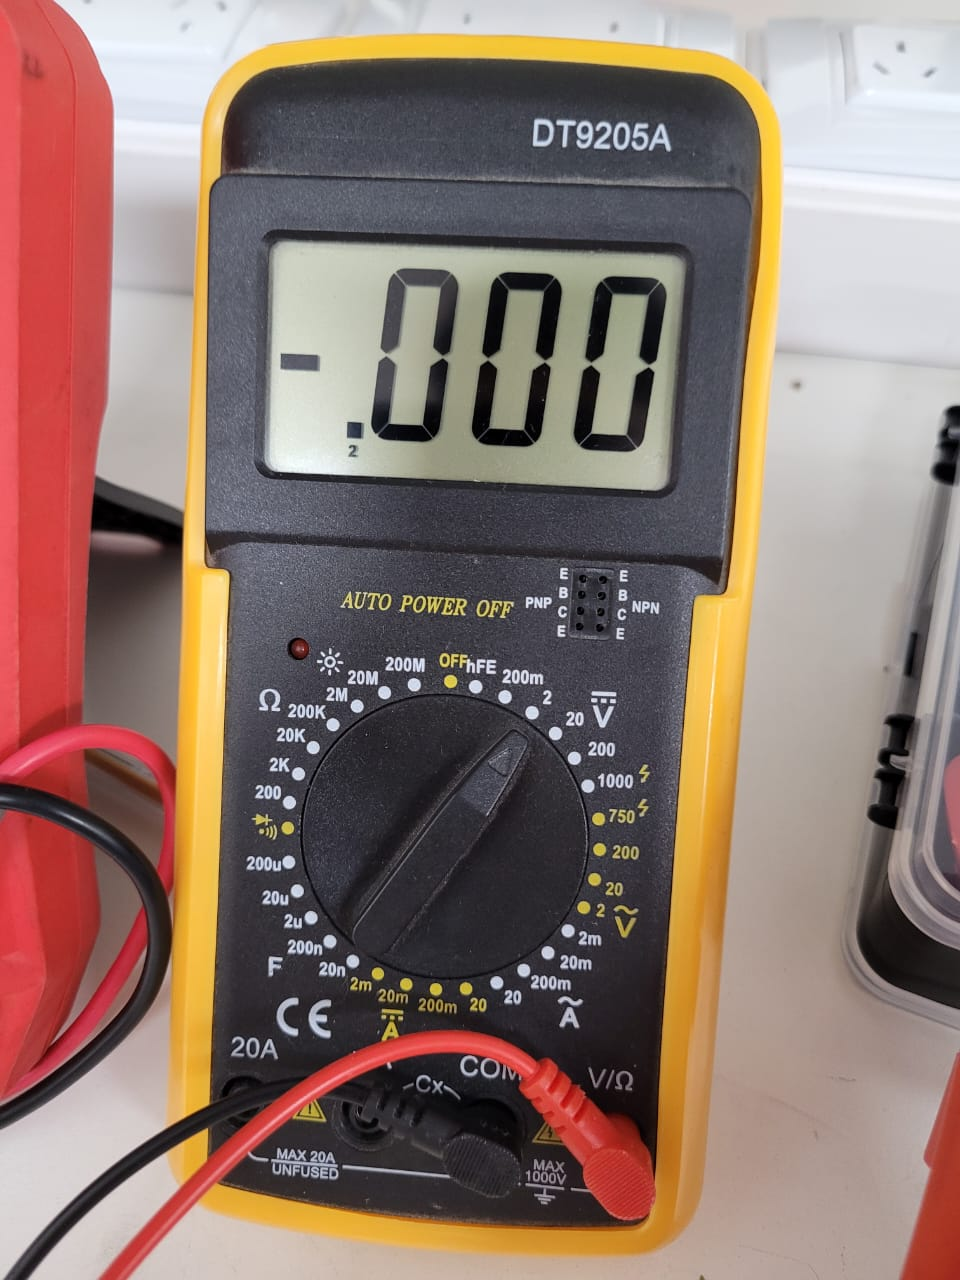
\includegraphics[width=\textwidth]{pictures/multimetro-angelo.jpeg}
            \caption{Instrumentos: multimétro digital Nº3, marca genérica modelo DT9205A.}
        \end{minipage}
    \end{figure}

    \subsection{Conclusión}
        Podemos concluir que las mediciones obtenidas en los correspondientes ensayos realizados en el laboratorio son los esperados. Estimamos ciertas desviaciones a causa de posibles errores de medición inherentes a los instrumentos utilizados y al factor humano. A pesar de ello, los resultados fueron satisfactorios y nos fue de gran utilidad para comprender el comportamiento de los diodos, y para desarrollar habilidades prácticas que nos serán útiles para futuros trabajos prácticos. 
    

\chapter{Comportamiento del diodo en función de la temperatura}

  El comportamiento eléctrico de los diodos semiconductores está fuertemente influenciado por la temperatura. Esto se
  debe a la dependencia de parámetros clave del dispositivo con respecto a la temperatura, como la corriente de saturación 
  inversa (\(I_S\)) y la tensión umbral de conducción directa.
  
  \section{Fundamento teórico}
  
    La ecuación característica de un diodo ideal es:
    
    \[
    I_D = I_S \left( e^{\frac{V_D}{n V_T}} - 1 \right)
    \]
    
    donde:
    \begin{itemize}
        \item \(I_D\) es la corriente que circula por el diodo,
        \item \(I_S\) es la corriente de saturación inversa,
        \item \(V_D\) es la tensión aplicada al diodo,
        \item \(n\) es el coeficiente de idealidad (típicamente entre 1 y 2),
        \item \(V_T = \frac{kT}{q}\) es la tensión térmica, que depende linealmente de la temperatura absoluta \(T\), con
            \(k\) siendo la constante de Boltzmann y \(q\) la carga del electrón.
    \end{itemize}
    
    A medida que la temperatura aumenta:
    \begin{enumerate}
        \item El valor de \(V_T\) también aumenta, lo cual afecta la pendiente de la curva \(I\)-\(V\).
        \item La corriente de saturación inversa \(I_S\) se incrementa exponencialmente con la temperatura, dado que 
            depende del número de portadores minoritarios generados térmicamente.
        \item Como consecuencia, la corriente para un mismo voltaje directo es mayor a temperaturas más altas.
        \item La tensión de umbral para que el diodo comience a conducir disminuye.
    \end{enumerate}
  
  \section{Simulación y análisis}
  
    Para observar este efecto, se ha realizado una simulación del diodo 1N3198 sometido a tres temperaturas distintas: 
    20 °C, 100 °C y 125 °C. El circuito simulado se muestra a continuación:
    
    \begin{figure}[H]
        \centering
        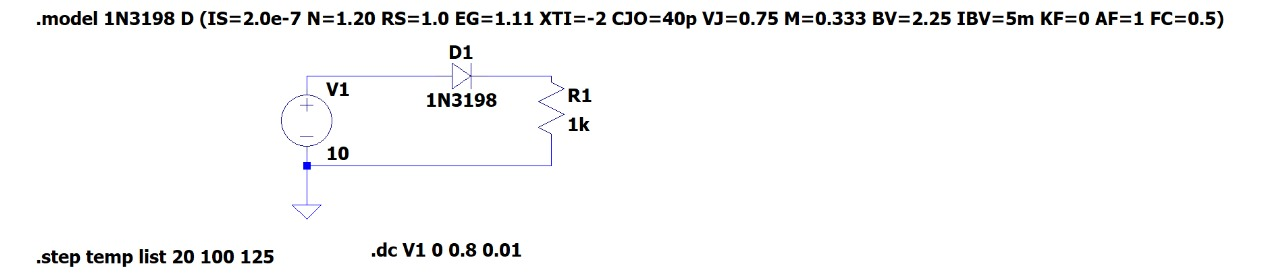
\includegraphics[width=0.7\textwidth]{pictures/comparacion_temperatura_circuito.jpeg}
        \caption{Circuito simulado para análisis de comportamiento térmico del diodo.}
    \end{figure}
    
    En la siguiente gráfica se puede observar cómo varía la curva característica corriente-voltaje del diodo en función de
    la temperatura:
    
    \begin{figure}[H]
        \centering
        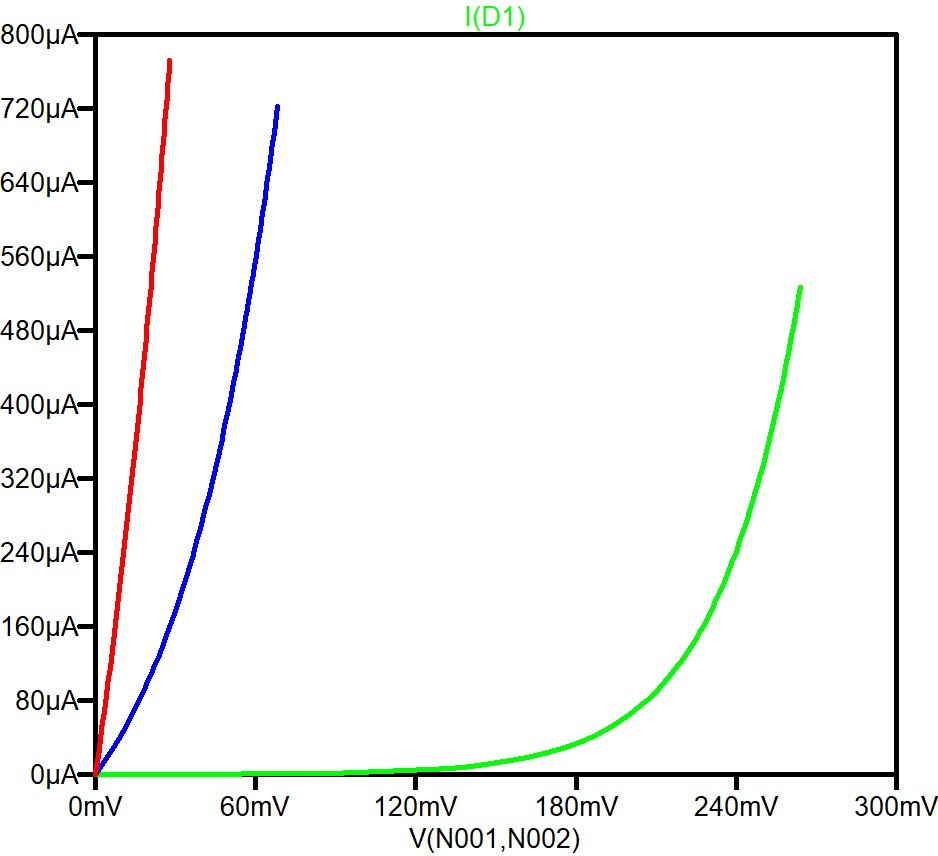
\includegraphics[width=0.6\textwidth]{pictures/comparacion_temperatura_grafico.jpeg}
        \caption{Curvas I-V del diodo 1N3198 a diferentes temperaturas. Curva roja: $125^|\circ C$; Curva azul:
            $100^\circ C$; Curva verde: $20^\circ C$}
    \end{figure}

    
    Como se puede apreciar, a mayor temperatura, la curva se desplaza hacia la izquierda, lo que indica que el diodo
    comienza a conducir a un menor voltaje. Además, para una misma tensión, la corriente que circula por el diodo es
    considerablemente mayor a temperaturas elevadas. Esta característica es clave en el diseño de circuitos electrónicos, 
    ya que una mala gestión térmica puede provocar corrientes excesivas no deseadas o incluso la destrucción del componente.


\chapter{Circuitos recortadores con diodos zener}

\section{Actividad de simulación}

\subsection*{Circuito a: Regulador de Voltaje con Zener}

\begin{itemize}
    \item \textbf{Objetivo:} Analizar el comportamiento de un circuito con diodo Zener como regulador de voltaje.
    \item \textbf{Simulación:} Se varía el voltaje de entrada \( V_{\text{in}} \) y se observa el comportamiento de la tensión de salida \( V_{\text{out}} \).
\end{itemize}

\subsubsection*{Esquema del circuito}
\begin{center}
    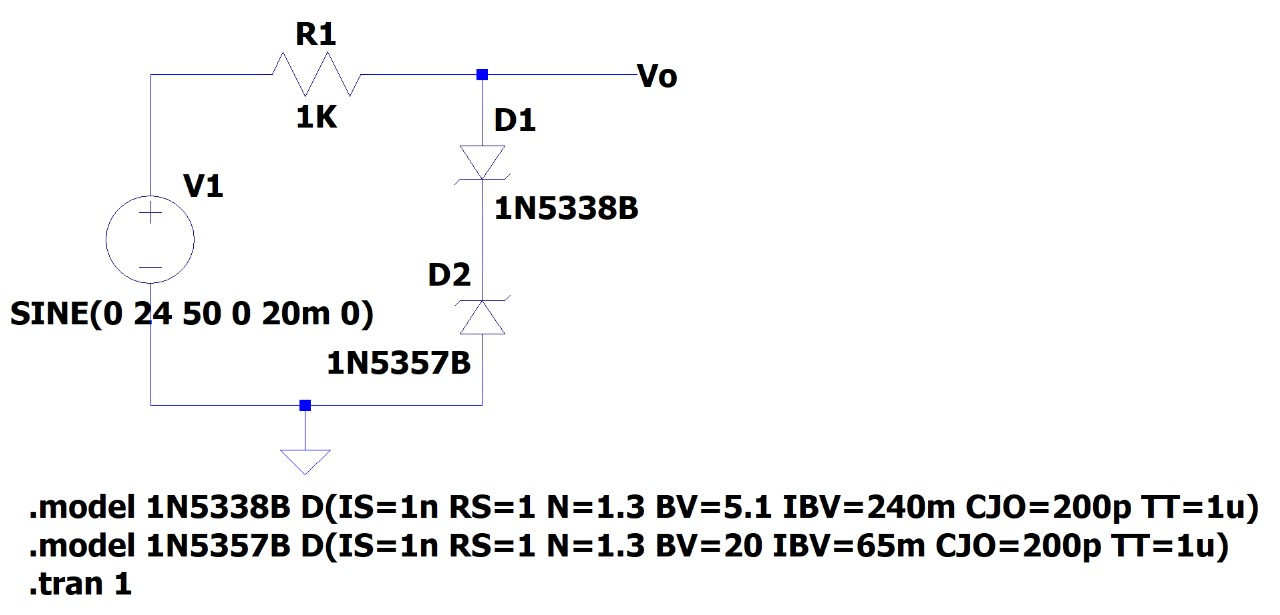
\includegraphics[width=0.5\textwidth]{pictures/zener_1_circuito.jpeg}
\end{center}

\subsubsection*{Análisis del comportamiento}

El diodo Zener se polariza en inversa. Su función principal es mantener la tensión de salida constante mientras el voltaje de entrada sea mayor que su tensión de ruptura \( V_Z \).

\begin{itemize}
    \item Si \( V_{\text{in}} < V_Z \), el diodo no conduce y \( V_{\text{out}} \approx V_{\text{in}} \).
    \item Si \( V_{\text{in}} \geq V_Z \), el diodo entra en conducción inversa (zona Zener) y mantiene \( V_{\text{out}} \approx V_Z \).
\end{itemize}

La corriente que circula por el diodo es:

\[
I_Z = \frac{V_{\text{in}} - V_Z}{R_s}
\]

\subsubsection*{Gráfico de simulación}
\begin{center}
    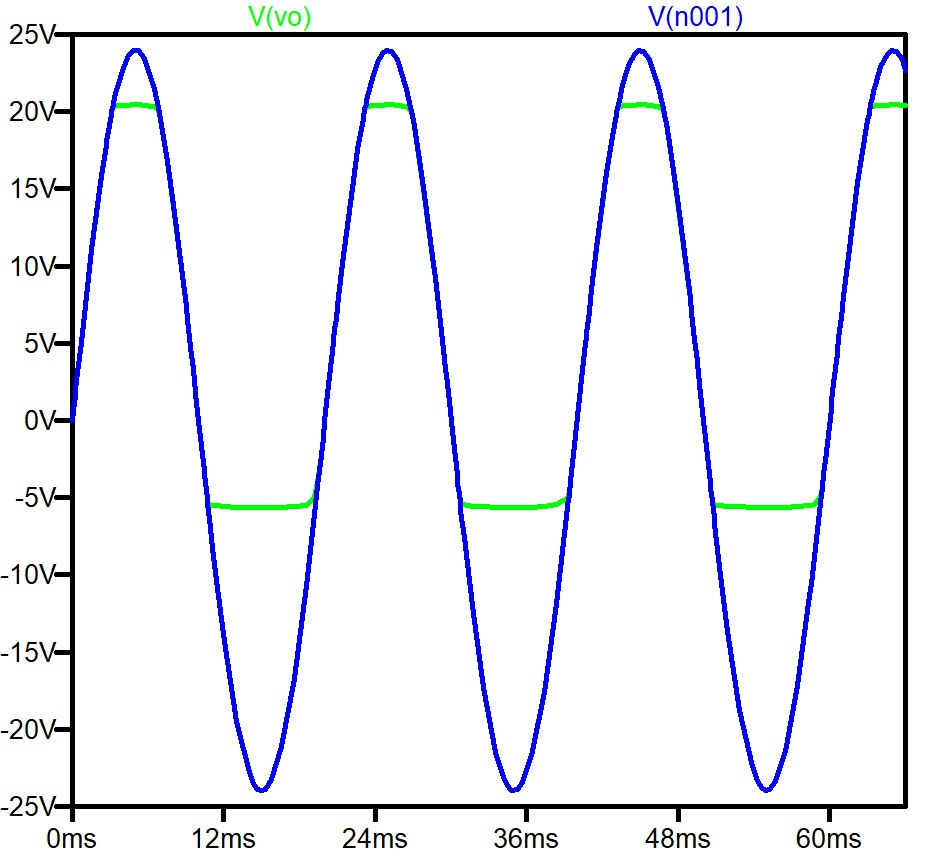
\includegraphics[width=0.6\textwidth]{pictures/zener_1_grafico.jpeg}
\end{center}

\noindent
El gráfico muestra cómo, a partir de cierta tensión, la salida se estabiliza en \( V_Z \), actuando como un recortador superior.


\subsection*{Circuito b: Recortador con Zener de diferente valor}

\begin{itemize}
    \item \textbf{Objetivo:} Observar el efecto de usar un diodo Zener con distinta tensión de ruptura.
\end{itemize}

\subsubsection*{Esquema del circuito}
\begin{center}
    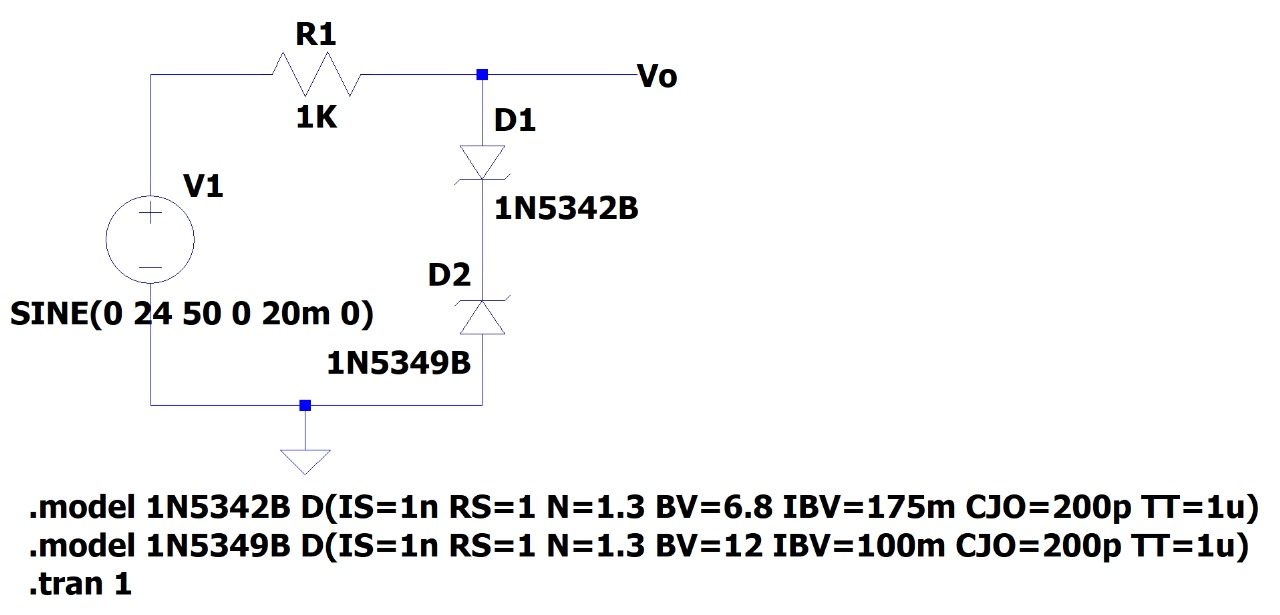
\includegraphics[width=0.5\textwidth]{pictures/zener_2_circuito.jpeg}
\end{center}

\subsubsection*{Análisis del comportamiento}

El principio de funcionamiento es el mismo que en el circuito anterior, pero se utiliza un diodo Zener con otra tensión de ruptura. El voltaje de salida se regula al nuevo valor \( V_Z' \).

\[
V_{\text{out}} =
\begin{cases}
    V_{\text{in}} & \text{si } V_{\text{in}} < V_Z' \\
    V_Z' & \text{si } V_{\text{in}} \geq V_Z'
\end{cases}
\]

\subsubsection*{Gráfico de simulación}
\begin{center}
    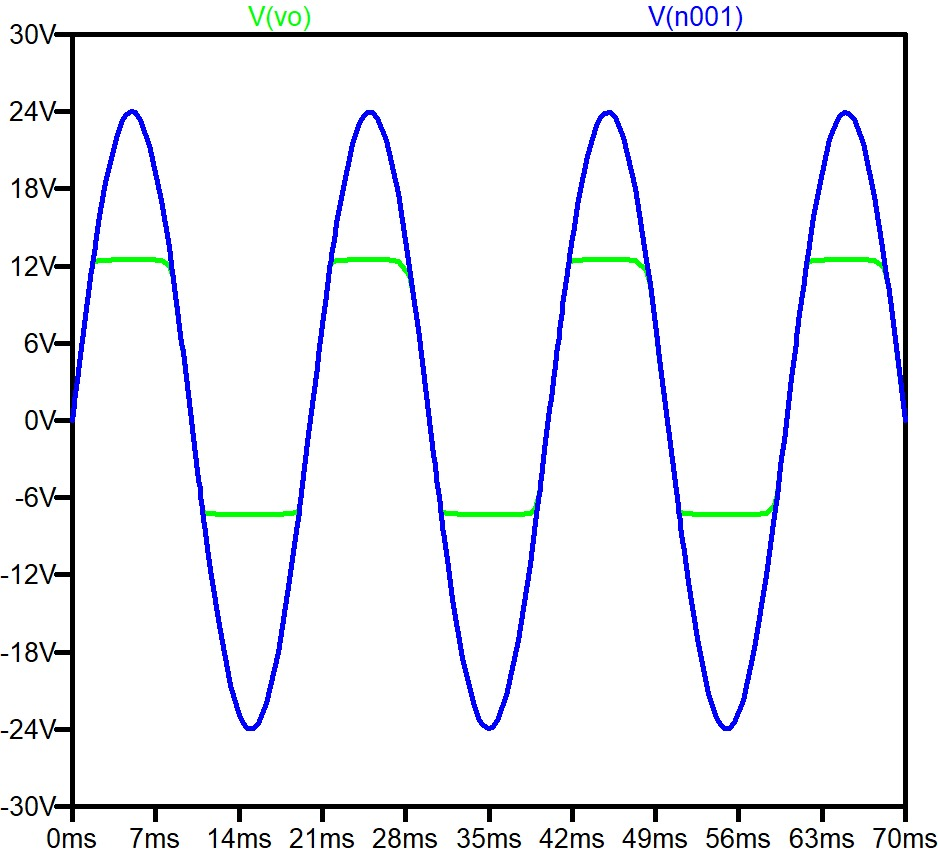
\includegraphics[width=0.6\textwidth]{pictures/zener_2_grafico.jpeg}
\end{center}

\noindent
Se observa un comportamiento similar, con la salida limitada a \( V_Z' \), actuando como recortador, pero en este caso con un umbral de corte distinto.

\subsection*{Conclusión}

Se comprobó que los diodos Zener permiten recortar el voltaje de salida una vez superado su valor de ruptura. Esto es útil para limitar la tensión en circuitos sensibles, estabilizar señales o implementar fuentes de voltaje fijo. Variar el tipo de diodo Zener modifica el umbral de recorte.

  
  \section{Actividad de laboratorio}

\subsection*{Procedimiento}

\begin{itemize}
    \item Calcular para cada uno de los circuitos propuestos el valor de la resistencia limitadora de corriente.
    \item Armar los circuitos propuestos, medir y graficar las señales de salida.
    \item Sacar las conclusiones de cada circuito.
\end{itemize}
    
    Para esta parte del trabajo practico se utilizaron los siguientes instrumentos:

    \begin{figure}[H]
    \centering
    \begin{minipage}{0.45\textwidth}
    \centering
    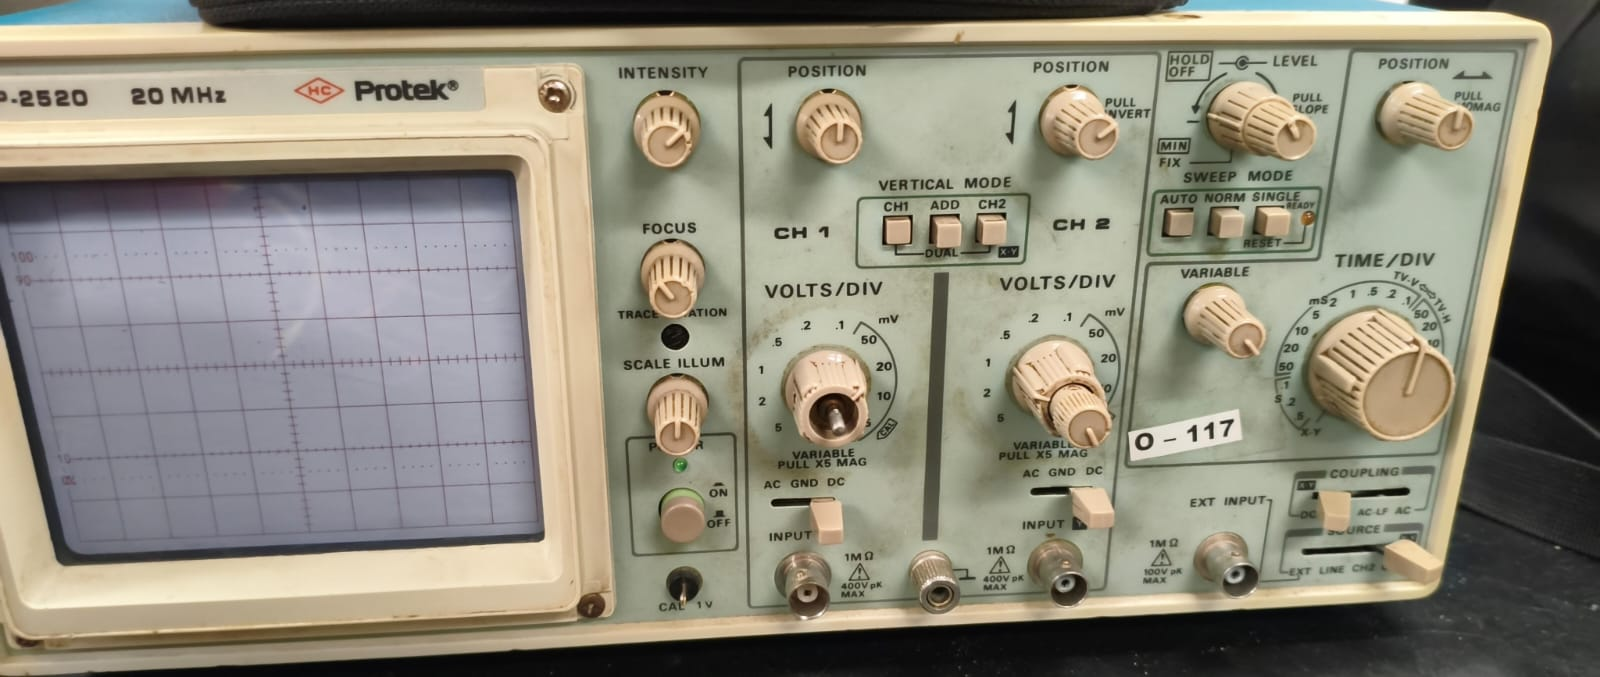
\includegraphics[width=\textwidth]{pictures/osciloscopio_utilizado_zener.jpeg}
    \caption{Numero de identificacion: O-117.}
    \end{minipage}
    \hspace{0.05\textwidth}
    \begin{minipage}{0.4\textwidth}
    \centering
    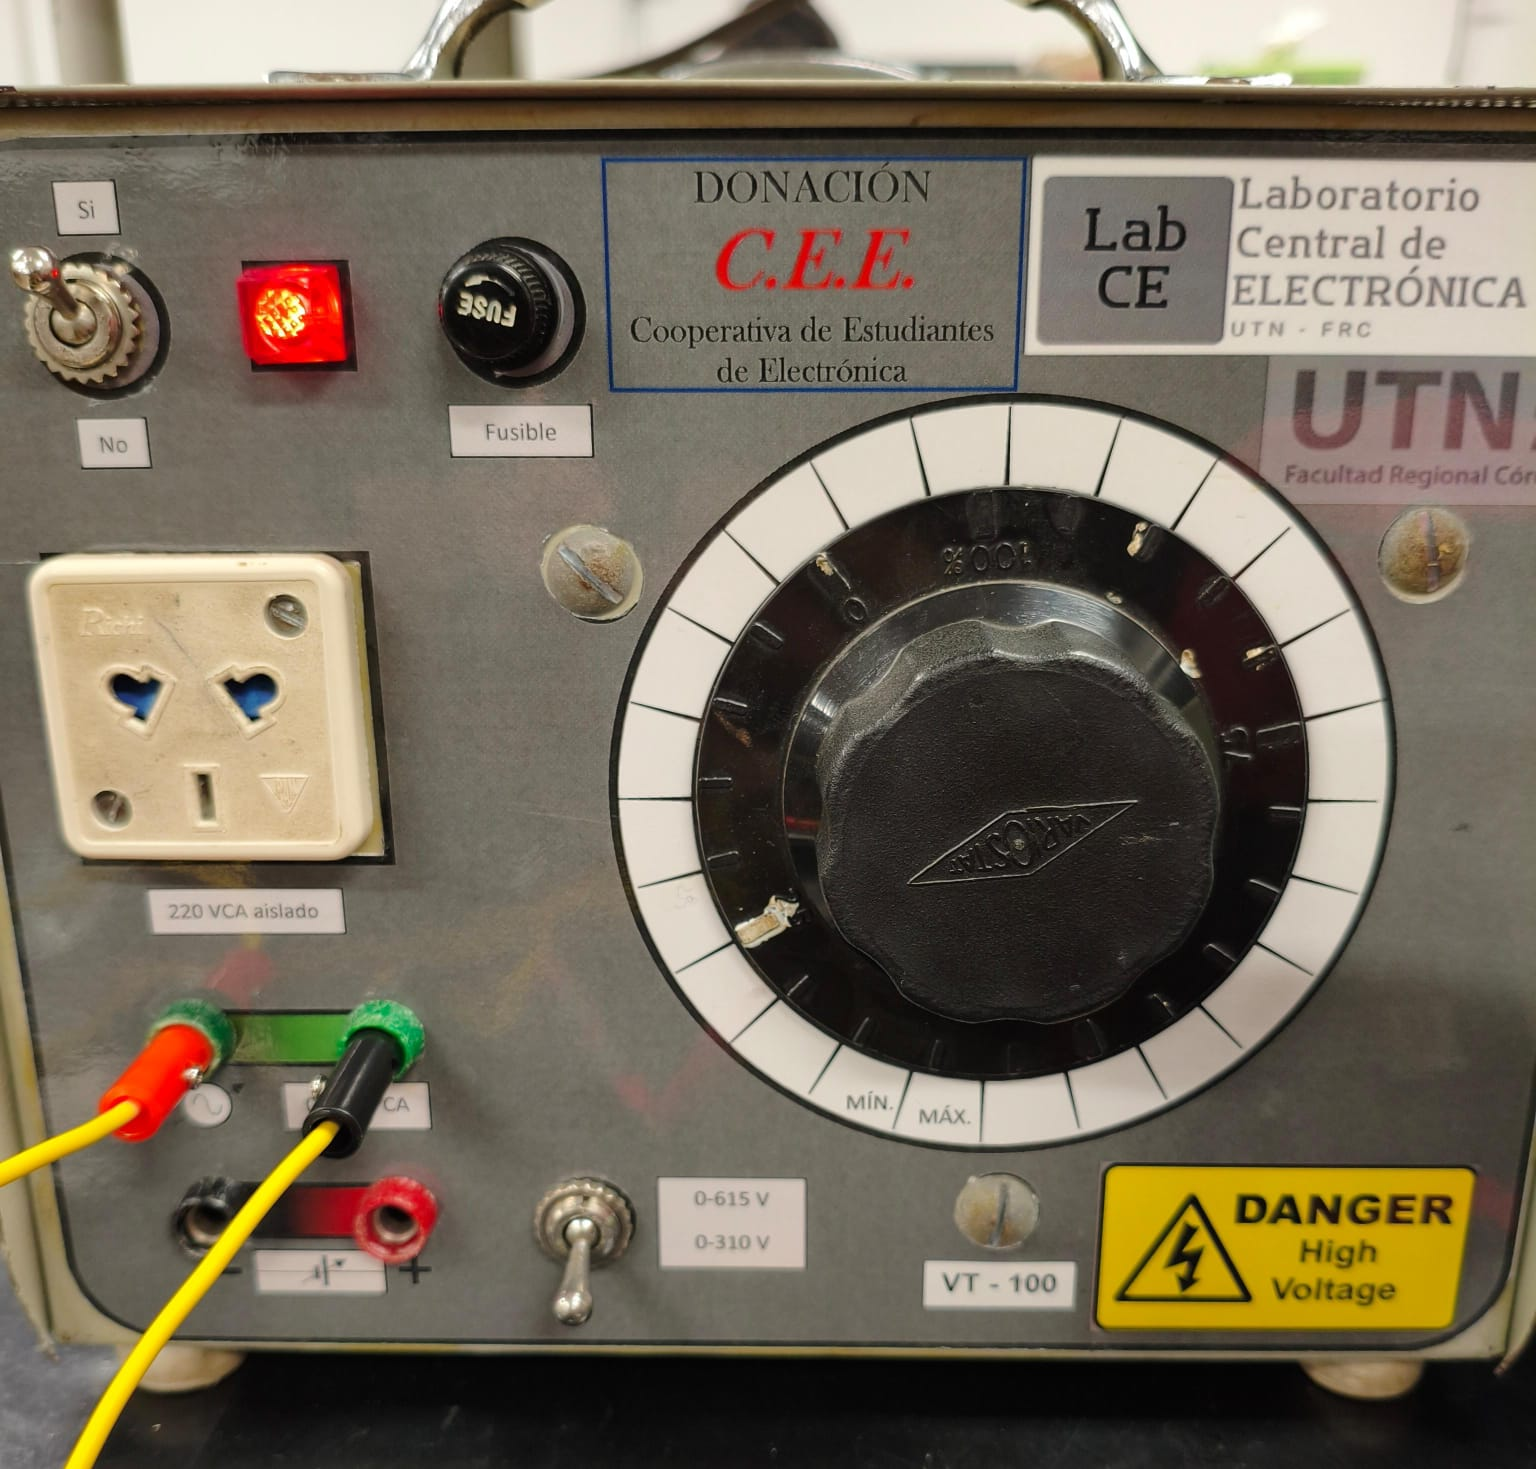
\includegraphics[width=\textwidth]{pictures/fuente_alterna_utilizada.jpeg}
    \caption{Numero de identificacion: VT-100.}
    \end{minipage}
    \end{figure}

    Luego se comprobo que la tension de la fuente fuera de $24 V_{ac}$.
    
    \begin{figure}[H]
        \centering
        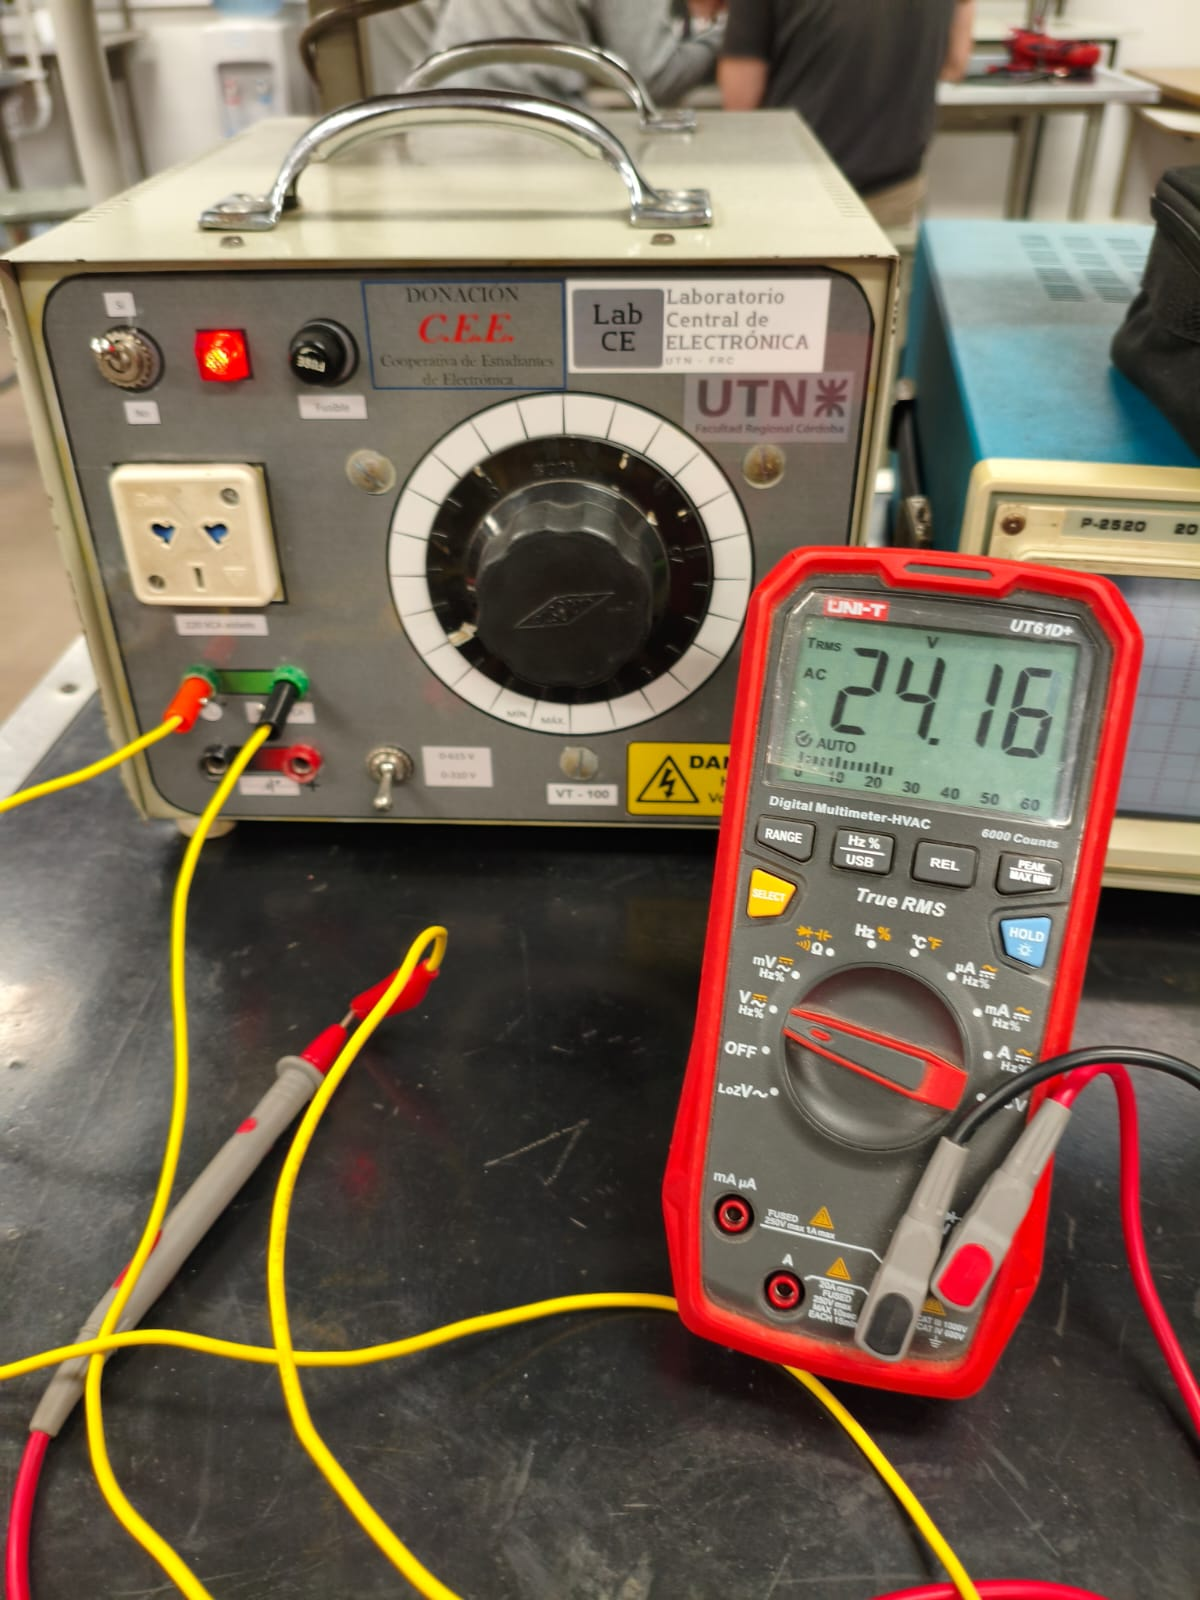
\includegraphics[width=0.5\textwidth]{pictures/tension_fuente_alterna.jpeg}
        \caption{Tension medida con un multimetro True RMS UNI-T UT61D+.}
    \end{figure}

    Para realizar las mediciones con el osciloscopio se utilizo una escala de tennsion de $5\V/div$ y una escala
    temporal de $2\text{ms}/div$.

 
    \begin{figure}[H]
        \centering
 \begin{minipage}{0.46\textwidth}
    \centering
        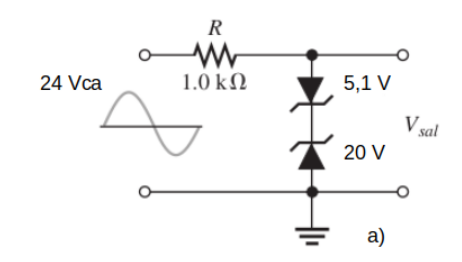
\includegraphics[width=\textwidth]{pictures/Esquematico_circuito_a.png}
        \caption{Esquematico del circuito A.}
    \end{minipage}
\hspace{0.05\textwidth}
\begin{minipage}{0.46\textwidth}
    \centering
        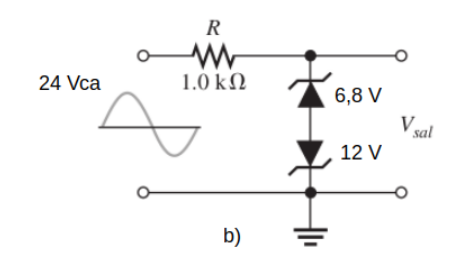
\includegraphics[width=\textwidth]{pictures/Esquematico_circuito_B.png}
        \caption{Esquematico del circuito B.}
    \end{minipage}
    \end{figure}

\subsection*{Circuito a)}
\begin{figure}[H]
    \centering
    \begin{minipage}{0.46\textwidth}
    \centering
    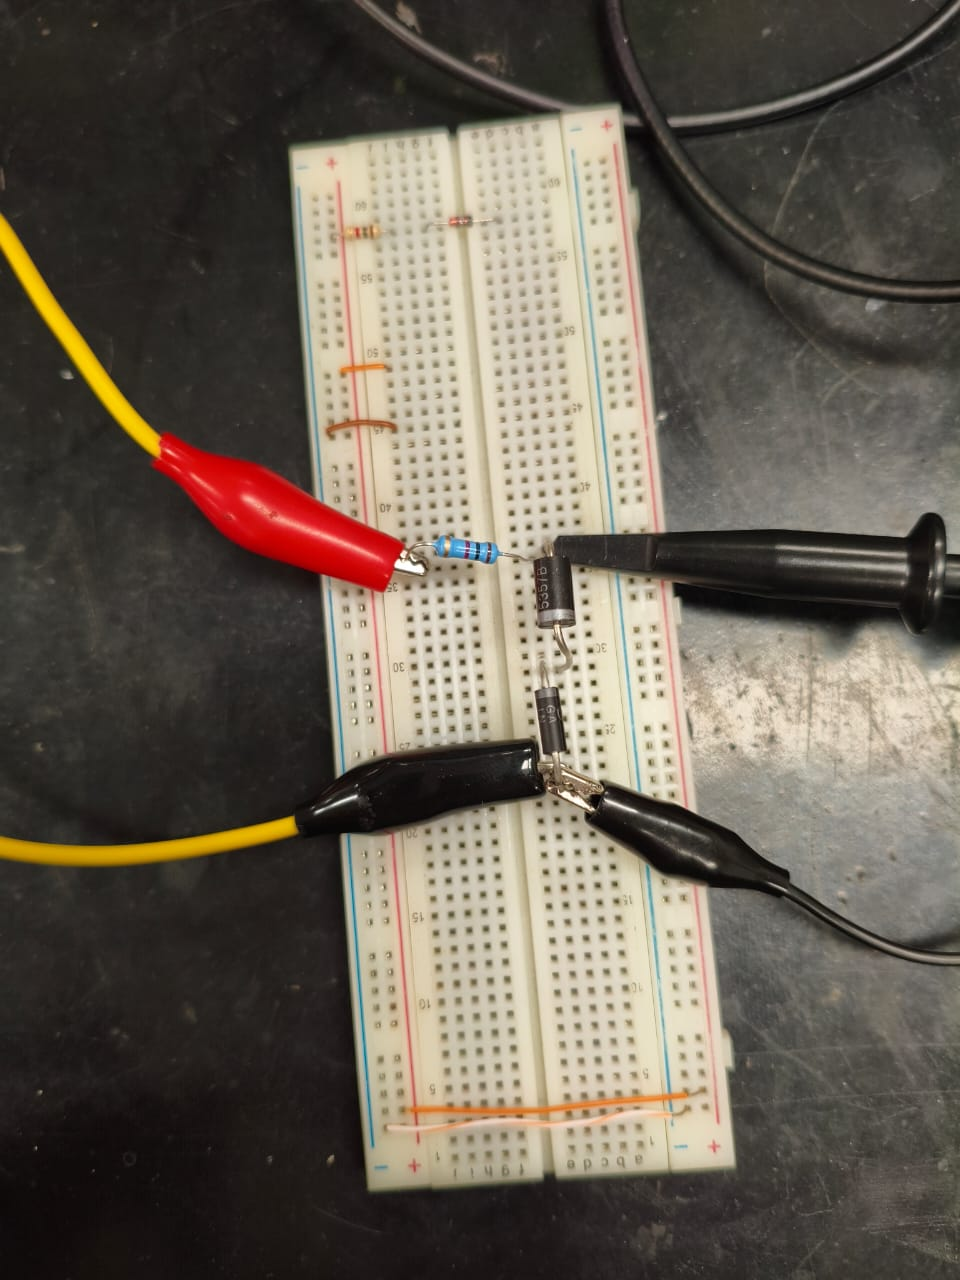
\includegraphics[width=\textwidth]{pictures/circuito_A.jpeg}
    \caption{Montaje en protoboard del circuito a).}
    En la foto, El diodo superior es el zener de $5.1\V$ y el diodo inferior es el zener de $20\V$.
\end{minipage}
\hspace{0.05\textwidth}
    \begin{minipage}{0.46\textwidth}
    \centering
    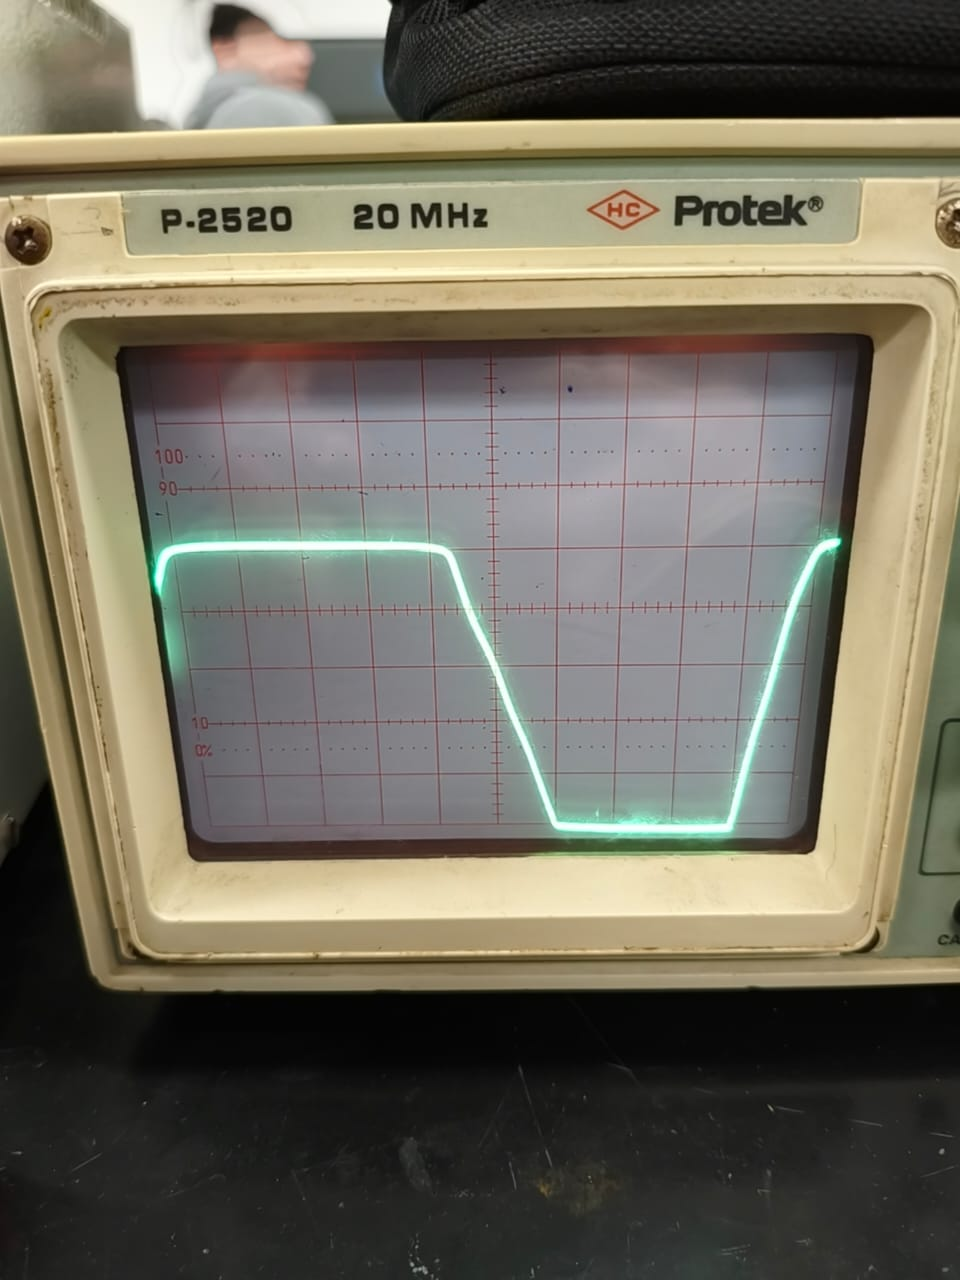
\includegraphics[width=\textwidth]{pictures/circuito_A_osciloscopio.jpeg}
    \caption{Señal de salida medida del circuito a).}
\end{minipage}
\end{figure}


\subsection*{Circuito b)}

\begin{figure}[H]
    \centering
    \begin{minipage}{0.46\textwidth}
    \centering
    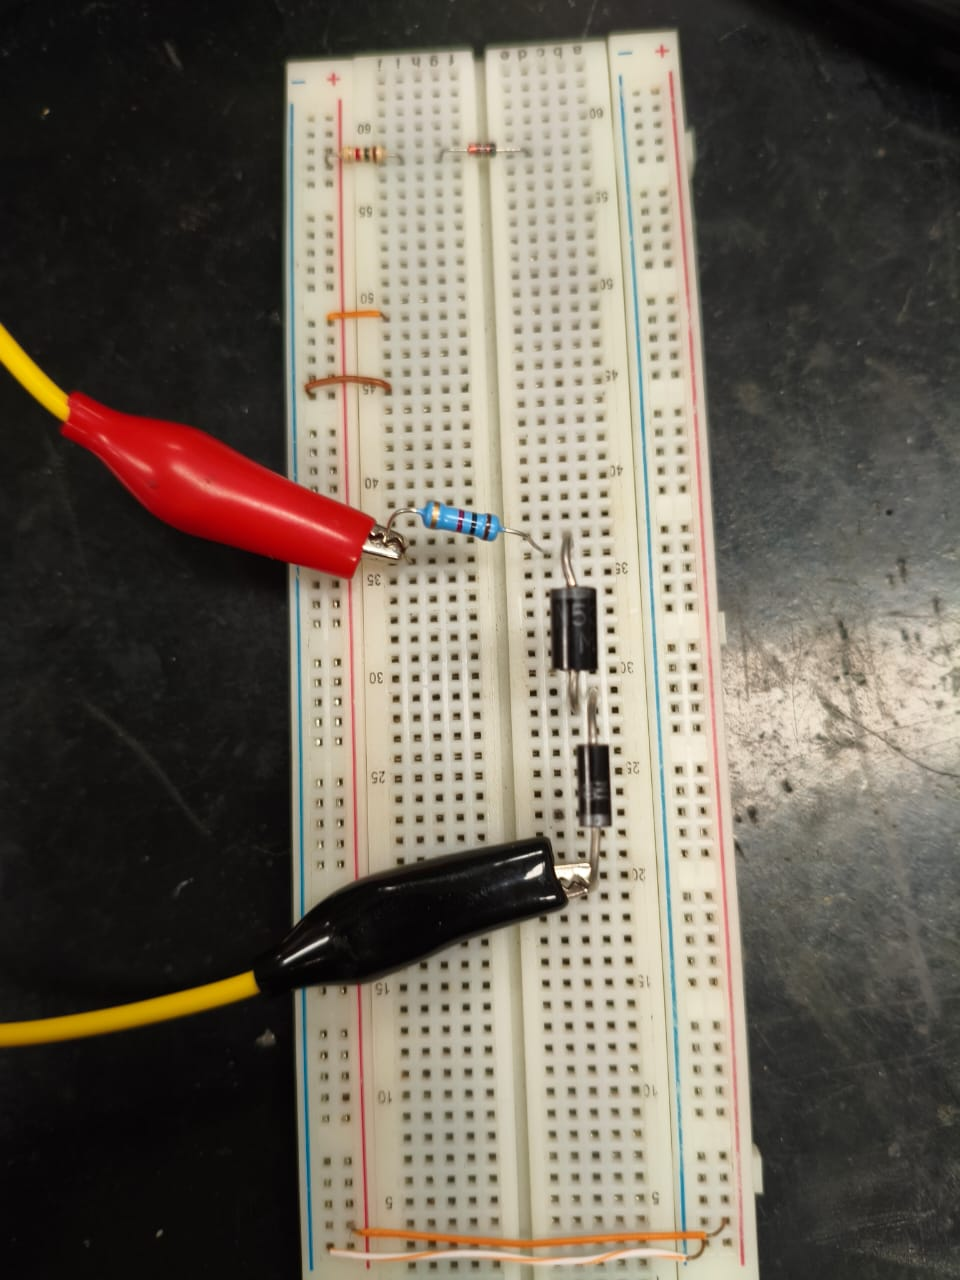
\includegraphics[width=\textwidth]{pictures/circuito_B.jpeg}
    \caption{Montaje en protoboard del circuito b).}
    En la foto, El diodo superior es el zener de $6.8\V$ y el diodo inferior es el zener de $12\V$.
\end{minipage}
\hspace{0.05\textwidth}
    \begin{minipage}{0.46\textwidth}
    \centering
    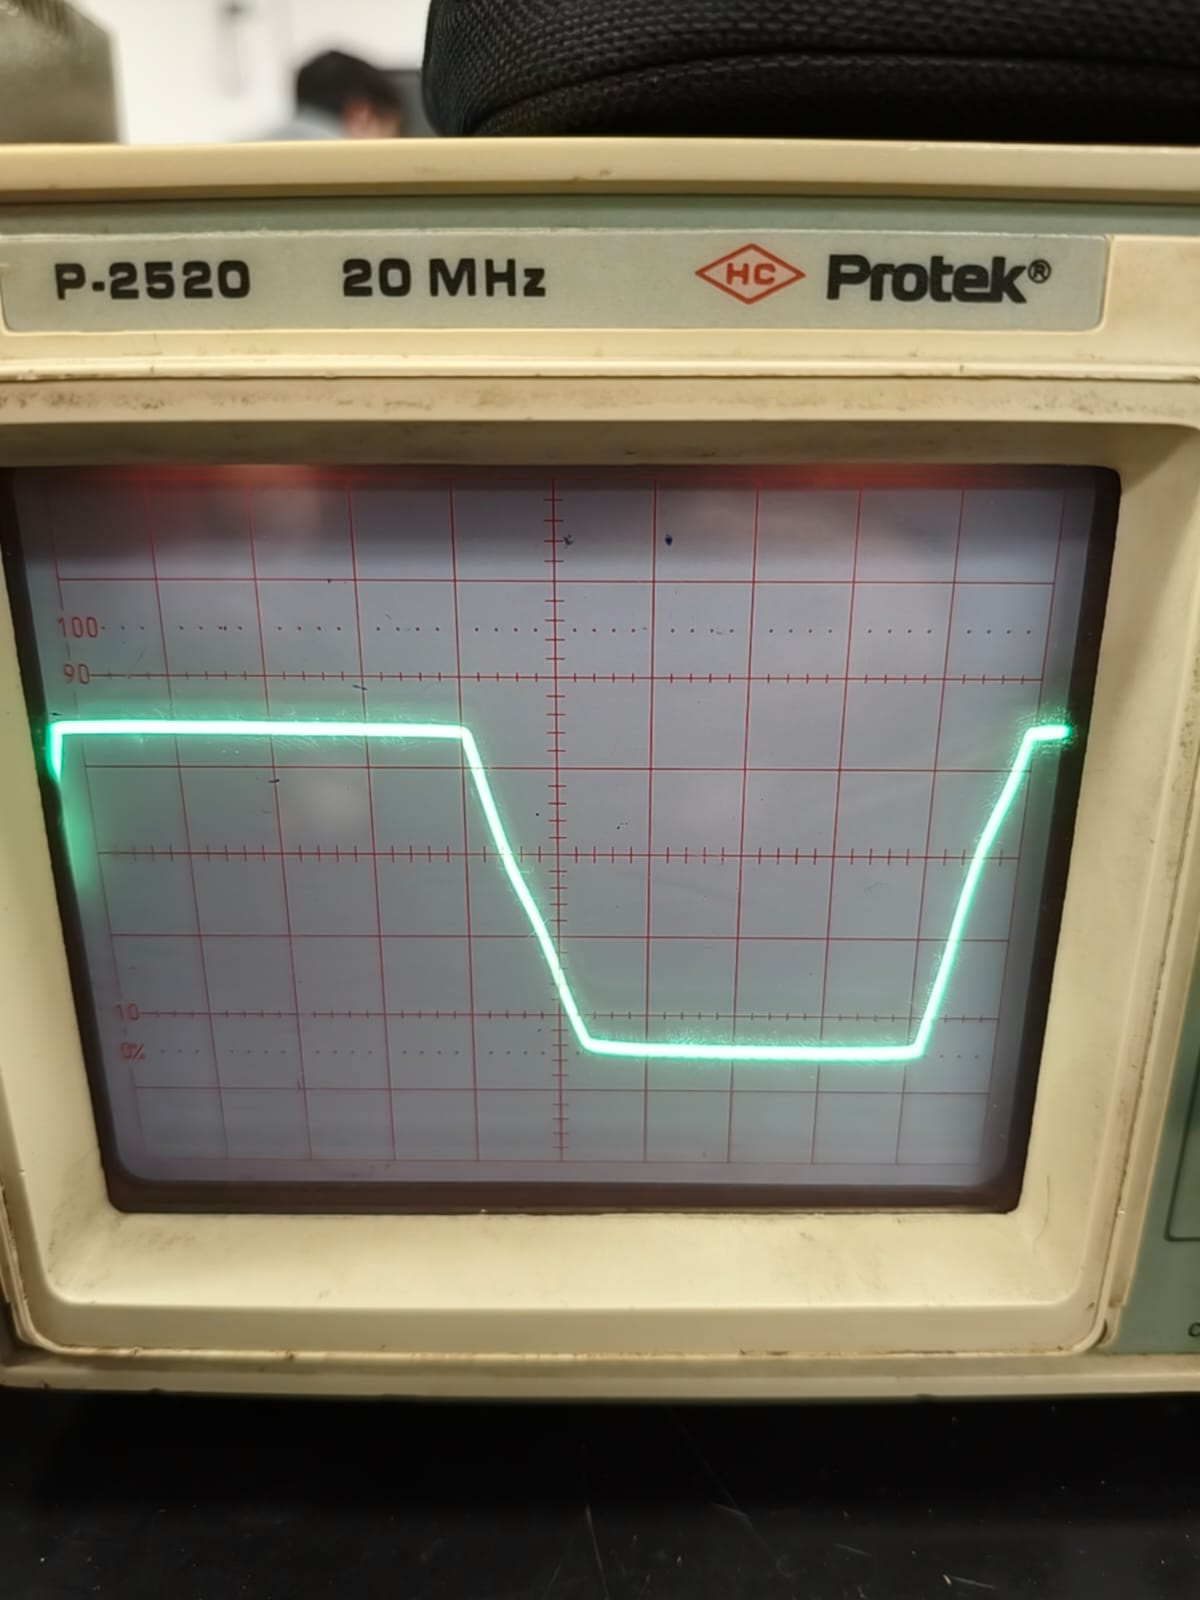
\includegraphics[width=\textwidth]{pictures/circuito_B_osciloscopio.jpeg}
    \caption{Señal de salida medida del circuito b).}
\end{minipage}
\end{figure}

\subsection*{Conclusiones}

\begin{itemize}
    \item Se confirmó que el diodo Zener actúa como recortador de voltaje cuando la señal supera su tensión de ruptura.
    \item En ambos circuitos, se pudo observar una clara limitación en la señal de salida, lo cual coincide con el análisis teórico y simulado.
    \item La comparación entre ambos circuitos permitió verificar el efecto de cambiar la tensión de ruptura del diodo Zener.
\end{itemize}
  

\chapter{Análisis sobre parámetros de hoja de datos}

  \section*{Características Eléctricas}
  
    \subsection*{Regímenes máximos}
      \begin{enumerate}
        \item $V_{RRM}$: Tensión repetitiva máxima en inversa. Es el máximo voltaje que se puede aplicar en polarización inversa de manera repetitiva sin dañar el dispositivo.
        \item $V_{RSM}$: Tensión máxima en inversa no repetitiva. Es el valor pico máximo que puede soportar el dispositivo en condiciones excepcionales.
        \item $I_{FRMS}$: Corriente eficaz directa máxima. Es la corriente RMS que el dispositivo puede conducir de forma continua sin sobrecalentamiento.
        \item $I_{FSM}$: Corriente de sobrecarga directa máxima. Es el valor pico máximo de corriente directa que puede soportar durante un pulso corto.
      \end{enumerate}
    
    \subsection*{Regímenes característicos}
      \begin{enumerate}
        \item $V_{BR}$: Tensión de ruptura. Es el voltaje en el cual el dispositivo comienza a conducir en inversa.
        \item $I_R$: Corriente de fuga inversa. Es la pequeña corriente que circula en inversa antes de la ruptura.
        \item $V_F$: Tensión de conducción directa. Es la caída de tensión directa cuando el dispositivo está conduciendo.
        \item $I_{RM}$: Corriente máxima en inversa. Es la máxima corriente que puede circular en polarización inversa antes de entrar en ruptura.
        \item $I_F$: Corriente directa. Es la corriente que circula a través del dispositivo cuando está polarizado en directa.
      \end{enumerate}
  
  \section*{Características Térmicas}
  
    \begin{enumerate}
        \item $T_J$: Temperatura de unión máxima. Es la temperatura máxima permitida en la unión del semiconductor durante su operación.
        \item $T_{STG}$: Temperatura de almacenamiento. Es el rango de temperatura dentro del cual se puede almacenar el dispositivo sin que sufra daños.
        \item $T_A$: Temperatura ambiente. Es la temperatura del entorno en el cual opera el dispositivo.
        \item $R_{\theta jc}$: Resistencia térmica unión-carcasa. Indica la resistencia al flujo de calor desde la unión interna del dispositivo hasta su encapsulado.
    \end{enumerate}
  
  \section*{Características de uso}
  
    \begin{enumerate}
        \item $V_{RMS}$: Tensión eficaz. Es el valor eficaz de la tensión alterna aplicada al dispositivo.
        \item $P_{tot}$: Potencia total disipada. Es la máxima potencia que el dispositivo puede disipar sin exceder los límites térmicos.
        \item $T_r$: Tiempo de recuperación. Es el tiempo que tarda el dispositivo en dejar de conducir una vez que se retira la señal de conducción.
    \end{enumerate}

  \chapter{Conclusión}

    A lo largo del trabajo se analizó el comportamiento característico de distintos tipos de diodos mediante simulaciones y mediciones prácticas de laboratorio. Se observó claramente la naturaleza no lineal de estos dispositivos, y se compararon sus respuestas según el material semiconductor —silicio o germanio— así como su funcionamiento en diversas configuraciones de circuito. También se evaluaron diodos Zener, comprobando su acción como limitadores de tensión al alcanzar su tensión de ruptura.

    Las simulaciones se mostraron útiles para anticipar el comportamiento del circuito, aunque se evidenció la importancia de seleccionar modelos precisos para obtener resultados confiables. Las mediciones en el laboratorio resultaron acordes a lo esperado, con pequeñas desviaciones atribuibles a factores instrumentales y externos.

    En particular, se confirmó la efectividad del diodo Zener para proteger y estabilizar señales en circuitos sensibles. La comparación entre distintos modelos permitió observar cómo varía el umbral de recorte según las especificaciones del componente. En conjunto, el trabajo permitió consolidar tanto los conocimientos teóricos como las habilidades prácticas necesarias para el análisis y diseño de circuitos electrónicos.
    
\end{document}
